\documentclass[a4paper,11pt]{article}
\usepackage[italian]{babel}
\usepackage[utf8]{inputenc}
\usepackage{graphicx}
\usepackage{epstopdf}
\usepackage[labelfont=bf]{caption}
\usepackage{adjustbox}
\usepackage{array}
\newcolumntype{M}[1]{>{\centering\arraybackslash}m{#1}}

\author{A.~Battistello\and P.~Ferretti}
\title{Machine Learning techniques to Model Data Intensive Application Performance}
\begin{document}
\maketitle
\tableofcontents
\section{Prime analisi}
\subsection{SVR vs Linear Regression}
Presa in considerazione la query R2, cerchiamo di prevedere il tempo di esecuzione della query con 80 cores.
Creeremo i nostri modelli facendo training su numeri di cores diversi da quello di test: 60, 72, 90, 100, 120. 
Dai risultati potremo confrontare la performance della regressione lineare rispetto a vari modelli di Support Vector Regression (lineare, polinomiale, sigmoidale). 
\newline
\newline
Come si può vedere dalla Tabella \ref{tabletest1} i risultati migliori si hanno dalla SVR lineare, mentre gli altri due tipi di SVR sono addirittura peggiori della semplice regressione lineare, probabilmente per problemi di \textit{overfit}.
\newline


\begin{table}[bhpt]
\centering
\begin{adjustbox}{center}
\begin{tabular}{c | c M{1.2cm} M{2.5cm} M{2.5cm} M{1.8cm}}
Modello & RMSE & R\textsuperscript{2} & Errore assoluto medio & Errore relativo medio & Differenza medie \tabularnewline
\hline
Regressione lineare & 0.0940 & 0.9952 & 213397 & 0.0295 & -0.0378 \\
SVR lineare & 0.0722 & 0.9991 & 220018 & 0.1730 & 0.0526\\
SVR polinomiale & 0.1050 & 0.9976 & 226093 & 0.1831 &0.0780\\
SVR sigmoidale & 0.5862 & 0.9802 & 279777 & 0.2286 & -0.2487
\end{tabular}
\end{adjustbox}
\\
\caption{Risultati per il primo test}
\label{tabletest1}
\end{table}


\begin {figure}[hbtp]
\centering
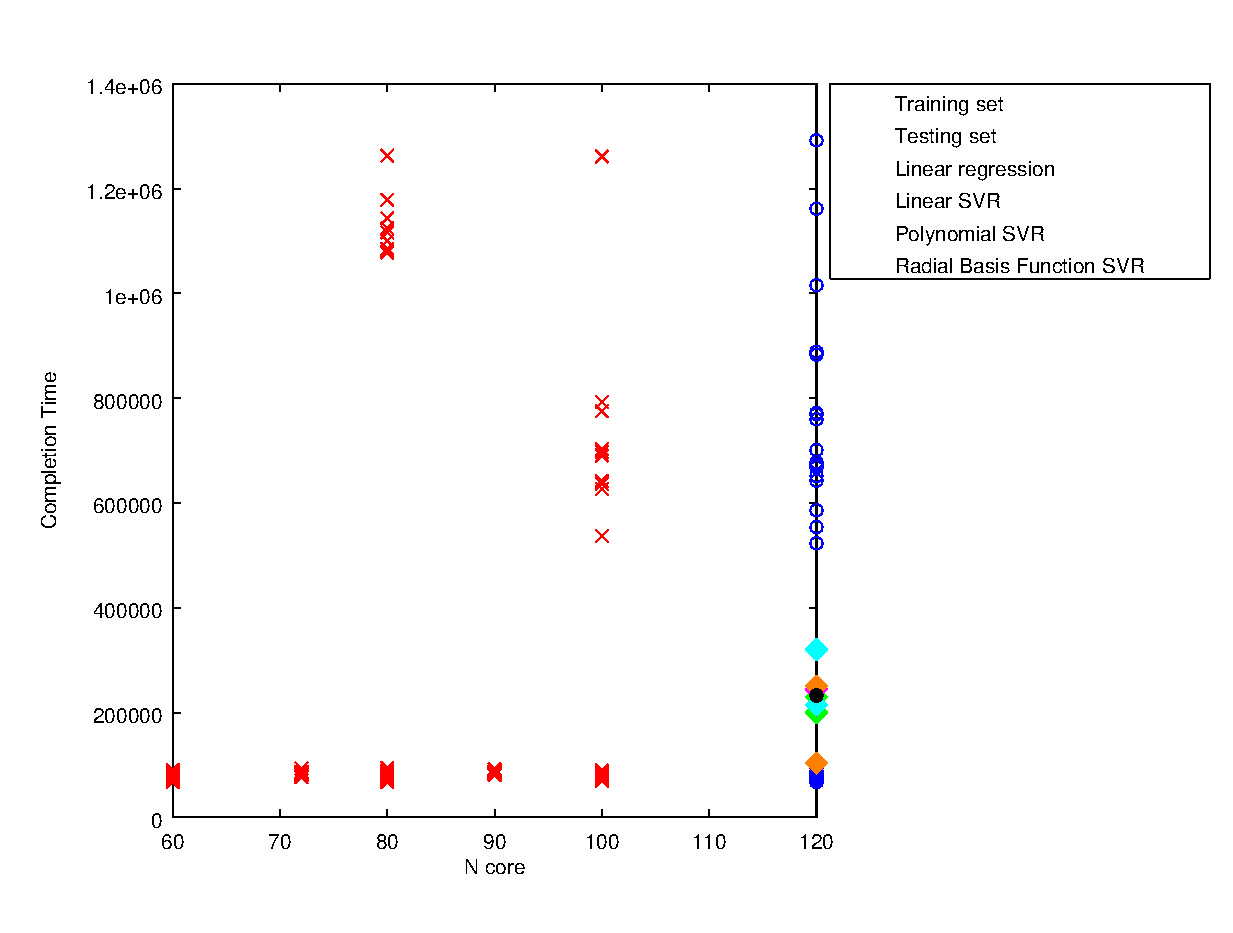
\includegraphics[width=\textwidth]{outputPlots/plot_Ncore.eps}
\caption {Test su numero di cores. La croce nera indica la media originale dei valori di test.}
\end {figure}

\newpage
\section{Features: solo nCores}
\subsection{Query R1 -- solo nCores}
\begin{table}[bhpt]
	\centering
	\begin{adjustbox}{center}
		\begin{tabular}{c | c M{1.2cm} M{2.5cm} M{2.5cm} M{1.8cm}}
			Modello & RMSE & R\textsuperscript{2} & Errore assoluto medio & Errore relativo medio \tabularnewline
			\hline
			Regressione lineare & 0.9214 & 0.1942 & 336910 & 4.7709 \\
			SVR lineare & 0.9428 & 0.1971 & 343224 & 5.3213 \\
			SVR polinomiale & 0.9460 & 0.2004 & 343757 & 6.2289 \\
			SVR sigmoidale & 0.9151 & 0.2592 & 336308 & 16.6191 \\
		\end{tabular}
	\end{adjustbox}
	\\
	\caption{Risultati per il test su query R1 
(solo nCores)}
	\label{table_R1_nCores}
\end{table}

\begin {figure}[hbtp]
\centering
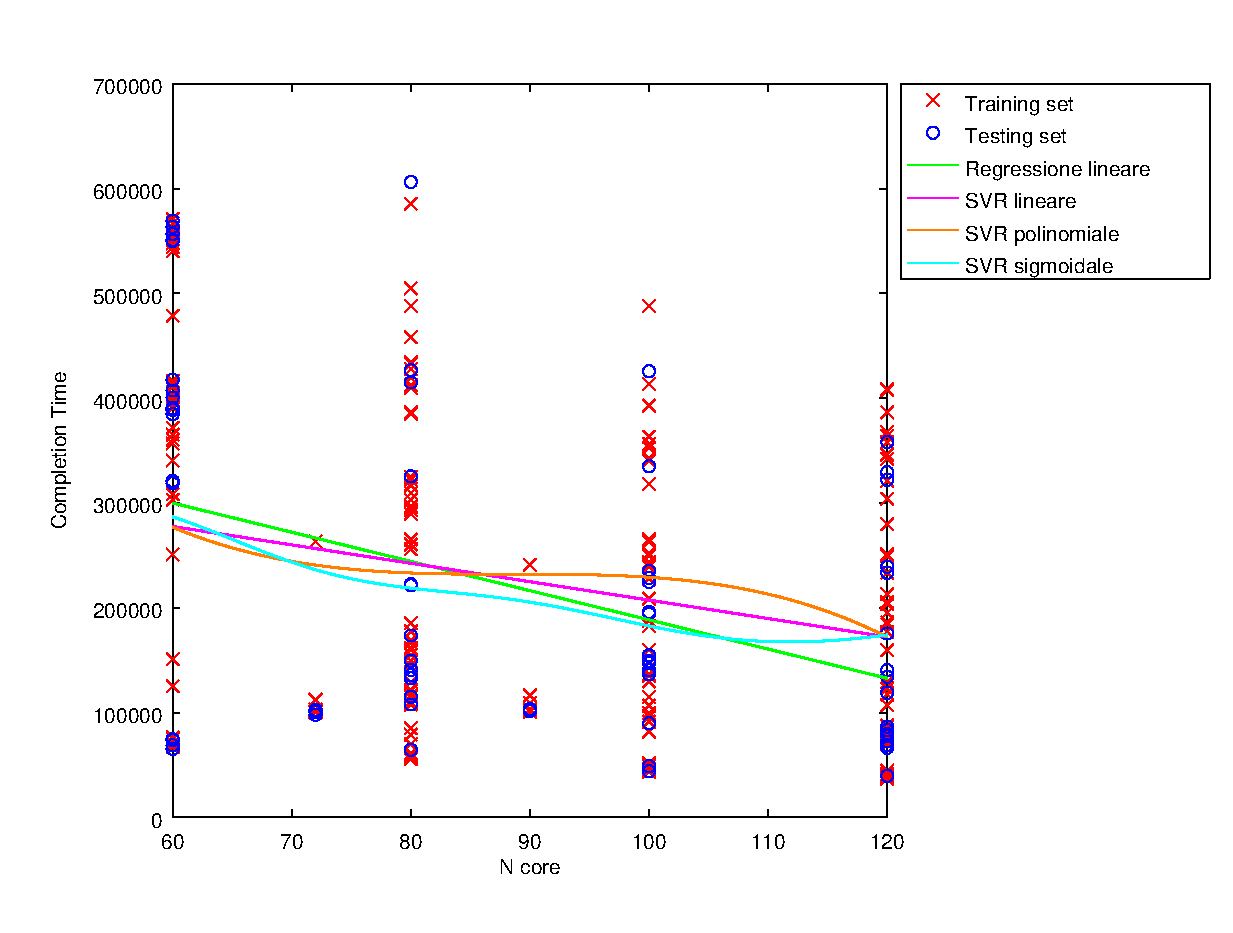
\includegraphics[width=\textwidth]{output/R1_SOLO_CORE/plot_R1_-.eps}
\caption {Completion time vs Numero di cores (query R1, solo nCores)}
\end {figure}

\newpage
\subsection{Query R2 -- solo nCores}
\begin{table}[bhpt]
	\centering
	\begin{adjustbox}{center}
		\begin{tabular}{c | c M{1.2cm} M{2.5cm} M{2.5cm} M{1.8cm}}
			Modello & RMSE & R\textsuperscript{2} & Errore assoluto medio & Errore relativo medio \tabularnewline
			\hline
			Regressione lineare & 1.0279 & 0.0011 &  83988 & 33.5075 \\
			SVR lineare & 1.0288 & 0.0038 &  83986 & 25.1568 \\
			SVR polinomiale & 1.0276 & 0.0053 &  83996 & 22.9335 \\
			SVR sigmoidale & 0.9861 & 0.0902 &  83660 & 5.3084 \\
		\end{tabular}
	\end{adjustbox}
	\\
	\caption{Risultati per il test su query R2 
(solo nCores)}
	\label{table_R2_nCores}
\end{table}

\begin {figure}[hbtp]
\centering
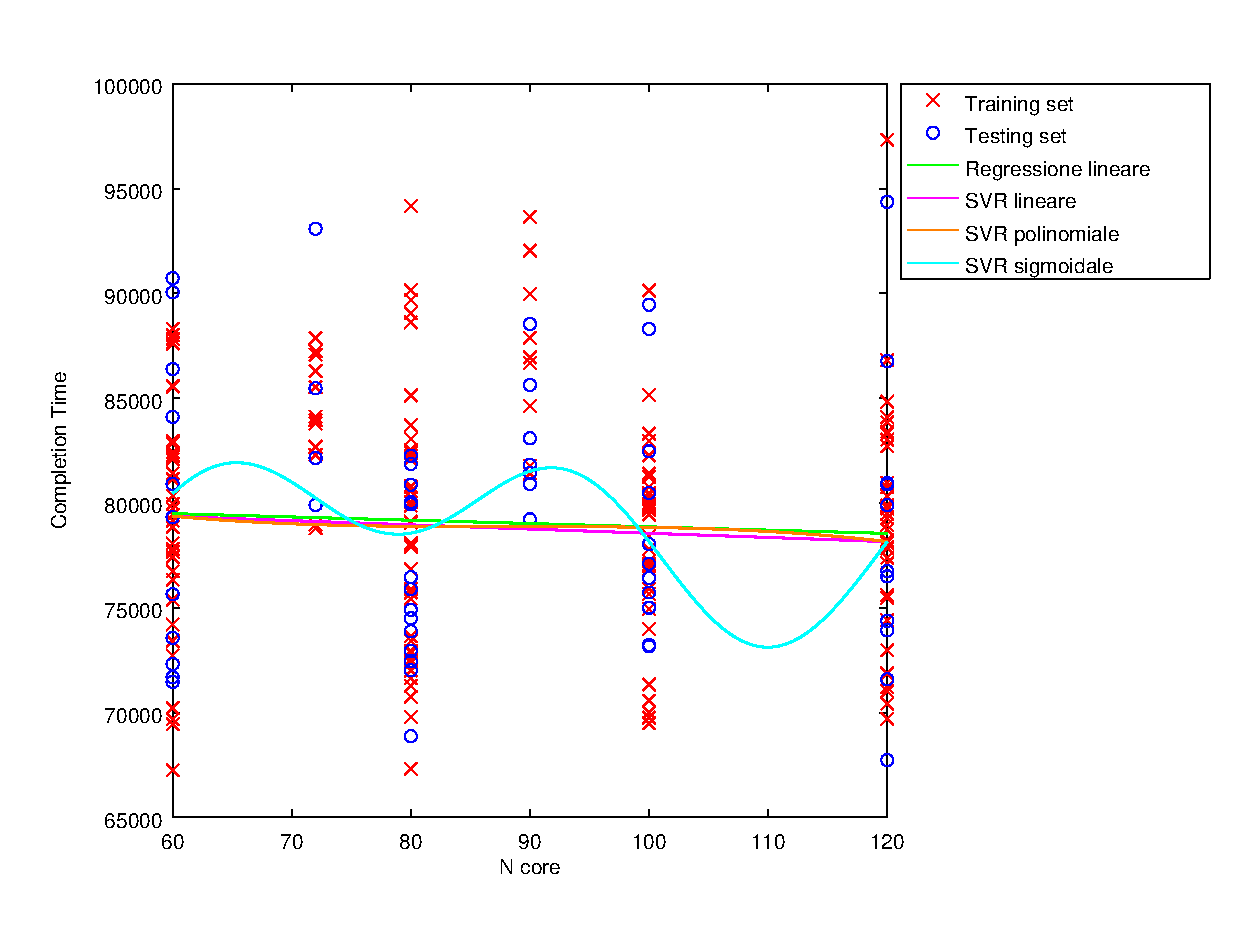
\includegraphics[width=\textwidth]{output/R2_SOLO_CORE_FILTER_500000/plot_R2_-.eps}
\caption {Completion time vs Numero di cores (query R2, solo nCores)}
\end {figure}

\newpage
\subsection{Query R3 -- solo nCores}
\begin{table}[bhpt]
	\centering
	\begin{adjustbox}{center}
		\begin{tabular}{c | c M{1.2cm} M{2.5cm} M{2.5cm} M{1.8cm}}
			Modello & RMSE & R\textsuperscript{2} & Errore assoluto medio & Errore relativo medio \tabularnewline
			\hline
			Regressione lineare & 0.8424 & 0.2186 & 857309 & 4.1395 \\
			SVR lineare & 0.8653 & 0.2198 & 865917 & 5.6068 \\
			SVR polinomiale & 0.8736 & 0.1973 & 867099 & 141.9124 \\
			SVR sigmoidale & 0.8479 & 0.3154 & 859635 & 5.9594 \\
		\end{tabular}
	\end{adjustbox}
	\\
	\caption{Risultati per il test su query R3 
(solo nCores)}
	\label{table_R3_nCores}
\end{table}

\begin {figure}[hbtp]
\centering
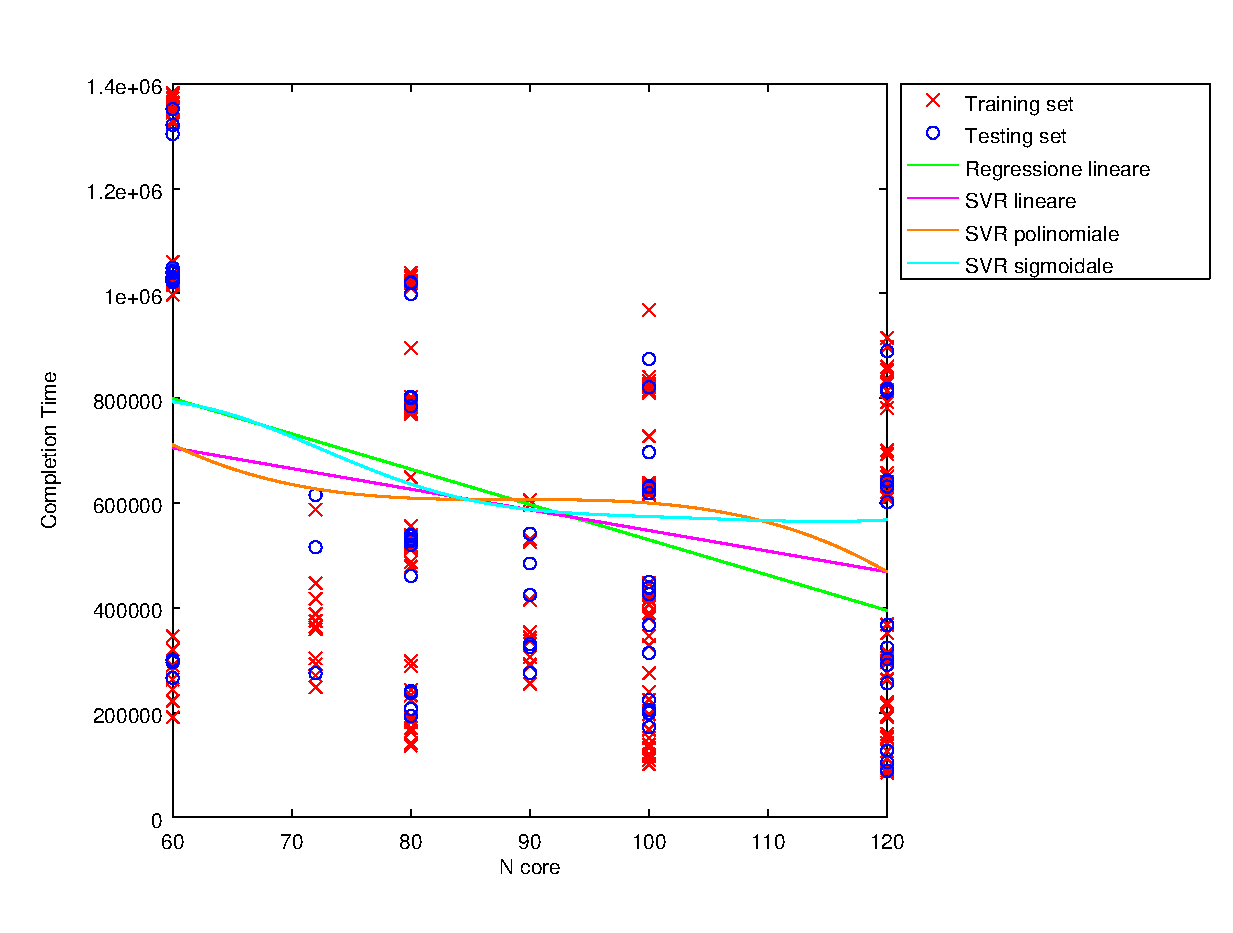
\includegraphics[width=\textwidth]{output/R3_SOLO_CORE/plot_R3_-.eps}
\caption {Completion time vs Numero di cores (query R3, solo nCores)}
\end {figure}

\newpage
\subsection{Query R4 -- solo nCores}
\begin{table}[bhpt]
	\centering
	\begin{adjustbox}{center}
		\begin{tabular}{c | c M{1.2cm} M{2.5cm} M{2.5cm} M{1.8cm}}
			Modello & RMSE & R\textsuperscript{2} & Errore assoluto medio & Errore relativo medio \tabularnewline
			\hline
			Regressione lineare & 0.7926 & 0.2278 & 667442 & 2.3770 \\
			SVR lineare & 0.7993 & 0.2307 & 669068 & 2.0618 \\
			SVR polinomiale & 0.8358 & 0.2111 & 666297 & 1.9794 \\
			SVR sigmoidale & 0.7923 & 0.2665 & 643343 & 1.7699 \\
		\end{tabular}
	\end{adjustbox}
	\\
	\caption{Completion time vs Numero di cores (query R4, solo nCores)}
	\label{table_R4_nCores}
\end{table}

\begin {figure}[hbtp]
\centering
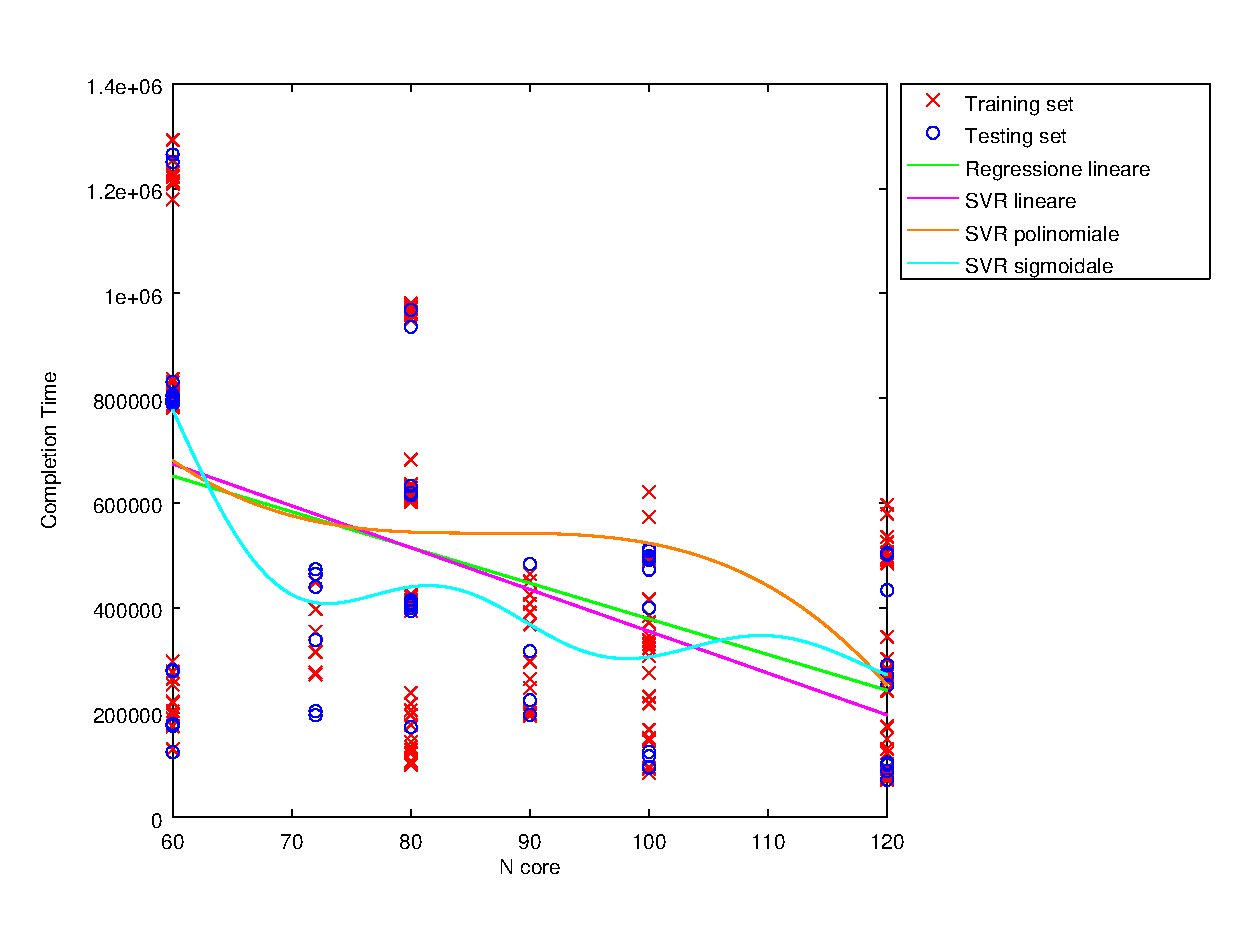
\includegraphics[width=\textwidth]{output/R4_SOLO_CORE_FILTER_1500000/plot_R4_-.eps}
\caption {Plot per il test su query R4 
(solo nCores)}
\end {figure}

\newpage
\subsection{Query R5 -- solo nCores}
\begin{table}[bhpt]
	\centering
	\begin{adjustbox}{center}
		\begin{tabular}{c | c M{1.2cm} M{2.5cm} M{2.5cm} M{1.8cm}}
			Modello & RMSE & R\textsuperscript{2} & Errore assoluto medio & Errore relativo medio \tabularnewline
			\hline
			Regressione lineare & 1.0607 & -0.0175 &  32694 & 9.4298 \\
			SVR lineare & 1.0595 & 0.0001 &  32728 & 13.2545 \\
			SVR polinomiale & 1.0654 & 0.0026 &  32786 & 98.7186 \\
			SVR sigmoidale & 1.0560 & 0.0009 &  32687 & 8.6378 \\
		\end{tabular}
	\end{adjustbox}
	\\
	\caption{Completion time vs Numero di cores (query R5, solo nCores)}
	\label{table_R5_nCores}
\end{table}

\begin {figure}[hbtp]
\centering
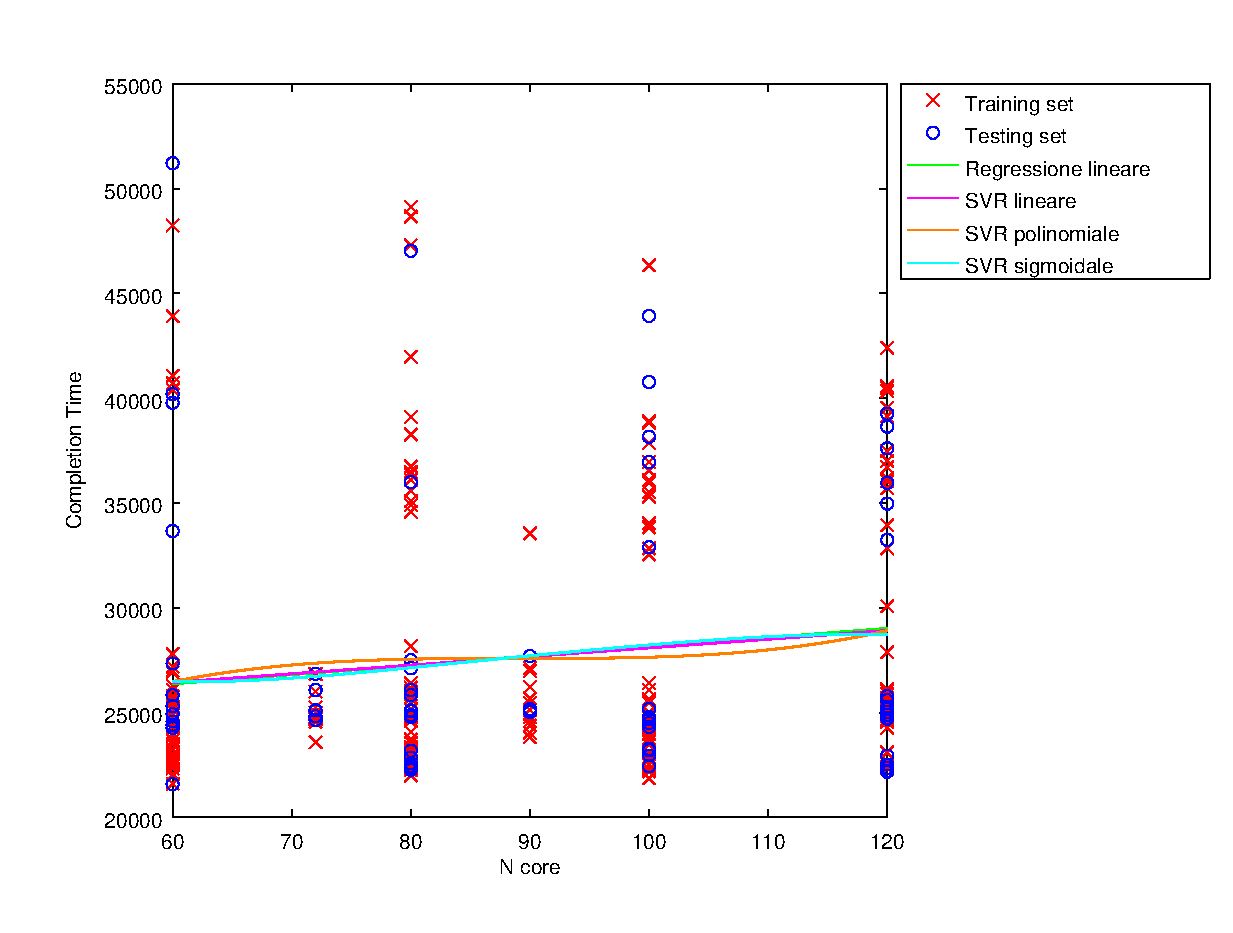
\includegraphics[width=\textwidth]{output/R5_SOLO_CORE/plot_R5_-.eps}
\caption {Plot per il test su query R5 
(solo nCores)}
\end {figure}

\newpage
\subsection{Confronto tra Query}

\begin {figure}[hbtp]
\centering
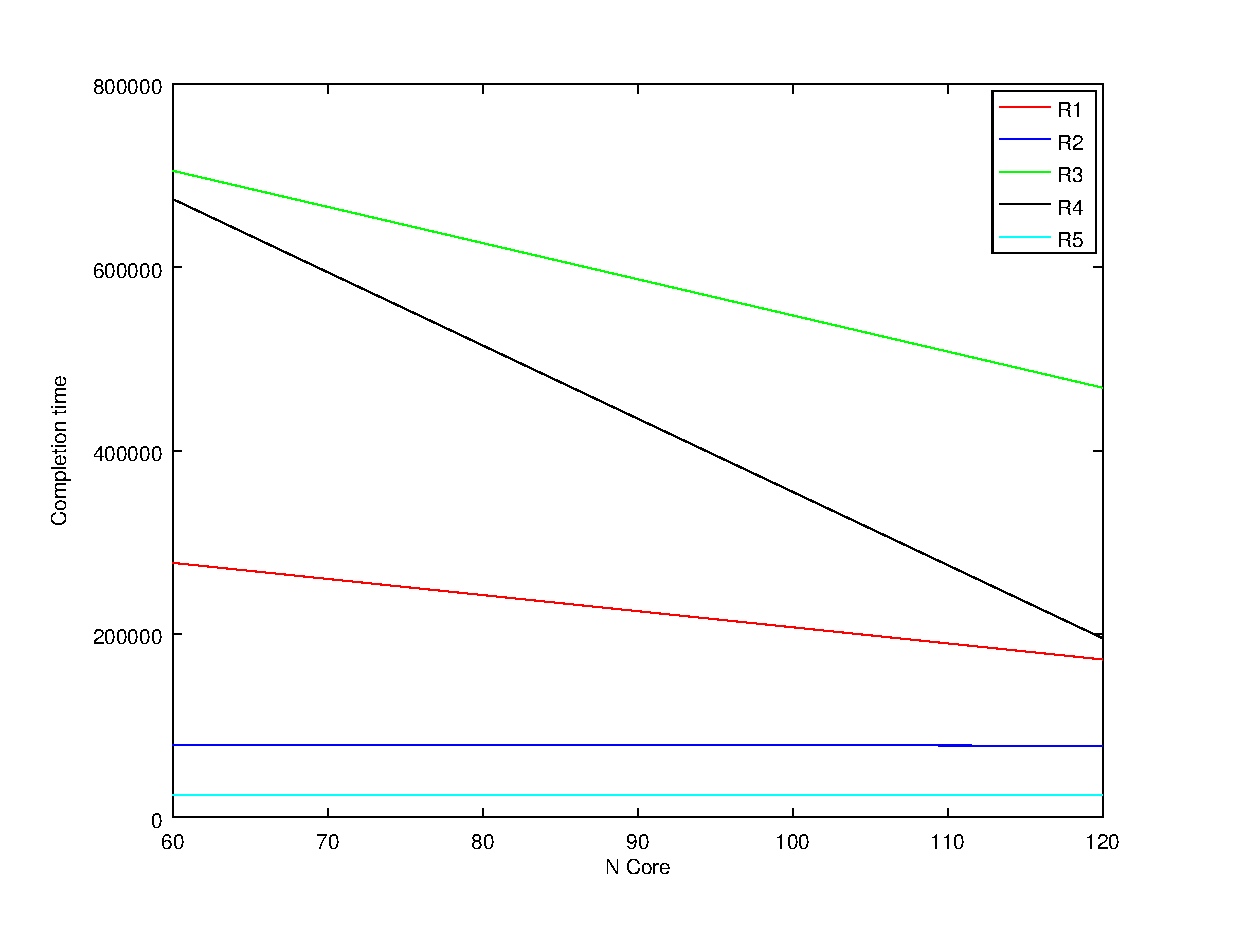
\includegraphics[width=\textwidth]{output/QUERY_COMP_CORE/SVRlineare/plot.eps}
\caption {Completion time vs Numero di core per ogni query (SVR lineare)}
\end {figure}

\newpage
\section{Features: solo Datasize}
\subsection{Query R1 -- solo Datasize}

\begin{table}[bhpt]
	\centering
	\begin{adjustbox}{center}
		\begin{tabular}{c | c M{1cm} M{2.5cm} M{2.5cm} M{1.8cm}}
			Modello & RMSE & R\textsuperscript{2} & Errore assoluto medio & Errore relativo medio \tabularnewline
			\hline
			Regressione lineare & 0.5954 & 0.6487 & 299905 & 0.8711 \\
			SVR lineare & 0.5995 & 0.6493 & 304265 & 0.9475 \\
			SVR polinomiale & 0.5782 & 0.6853 & 306565 & 3.3077 \\
			SVR sigmoidale & 0.5891 & 0.6609 & 298098 & 1.0758 \\
		\end{tabular}
	\end{adjustbox}
	\\
	\caption{Risultati per il test su query R1 (solo Datasize)}
	\label{table_R1_datasize}
\end{table}

\begin {figure}[hbtp]
\centering
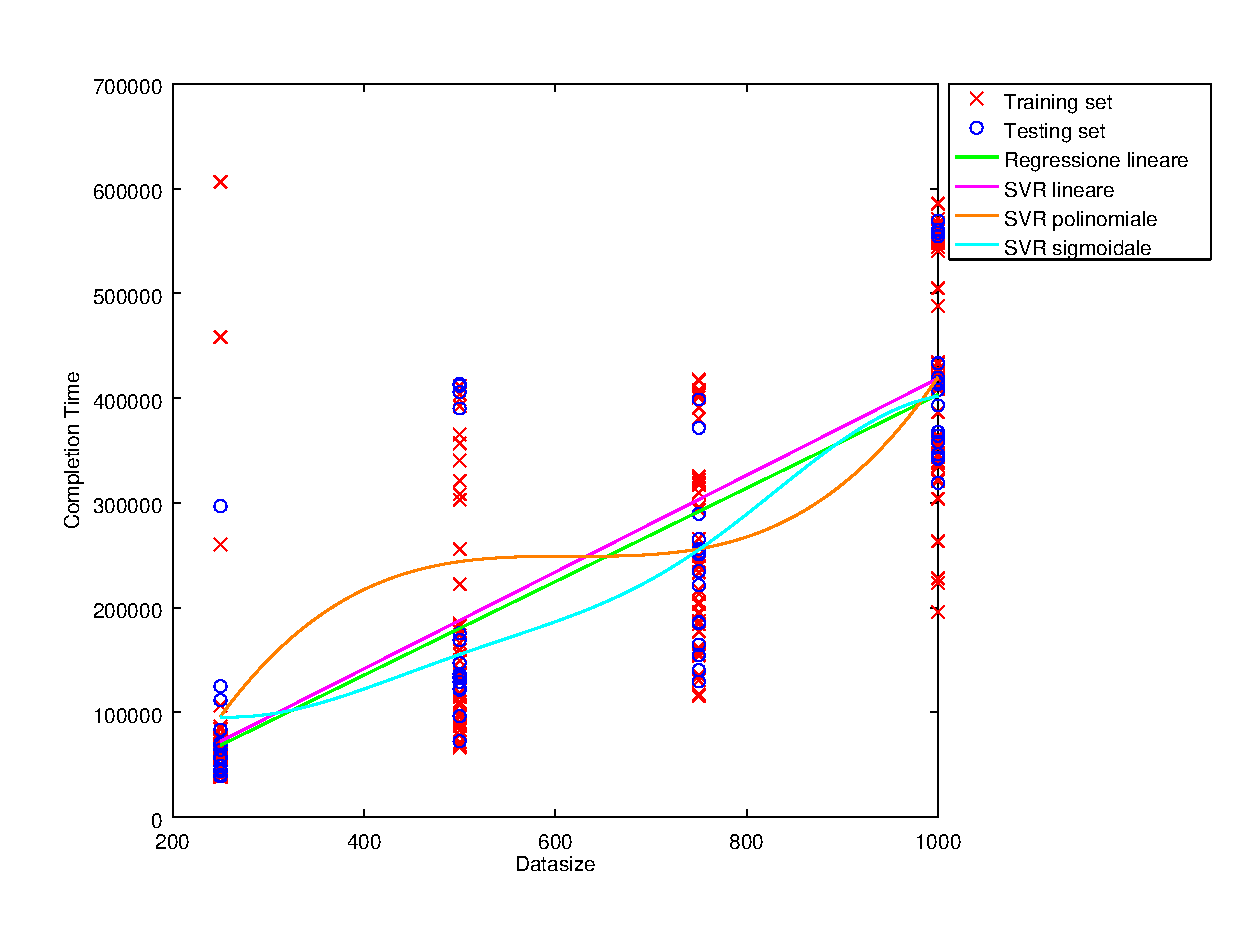
\includegraphics[width=\textwidth]{output/R1_SOLO_DATASIZE/plot_R1.eps}
\caption {Completion time vs Datasize (query R1, solo Datasize)}
\end {figure}

\newpage
\subsection{Query R2 -- solo Datasize}
\begin{table}[bhpt]
	\centering
	\begin{adjustbox}{center}
		\begin{tabular}{c | c M{1cm} M{2.5cm} M{2.5cm} M{1.8cm}}
			Modello & RMSE & R\textsuperscript{2} & Errore assoluto medio & Errore relativo medio \tabularnewline
			\hline
			Regressione lineare & 0.7694 & 0.4398 & 425310 & 1.3569 \\
			SVR lineare & 0.7690 & 0.4437 & 419702 & 1.2363 \\
			SVR polinomiale & 0.5527 & 0.7148 & 366820 & 4.3320 \\
			SVR sigmoidale & 0.4320 & 0.8241 & 299461 & 0.2465 \\
		\end{tabular}
	\end{adjustbox}
	\\
	\caption{Risultati per il test su query R2 (solo Datasize)}
	\label{table_R2_datasize}
\end{table}

\begin {figure}[hbtp]
\centering
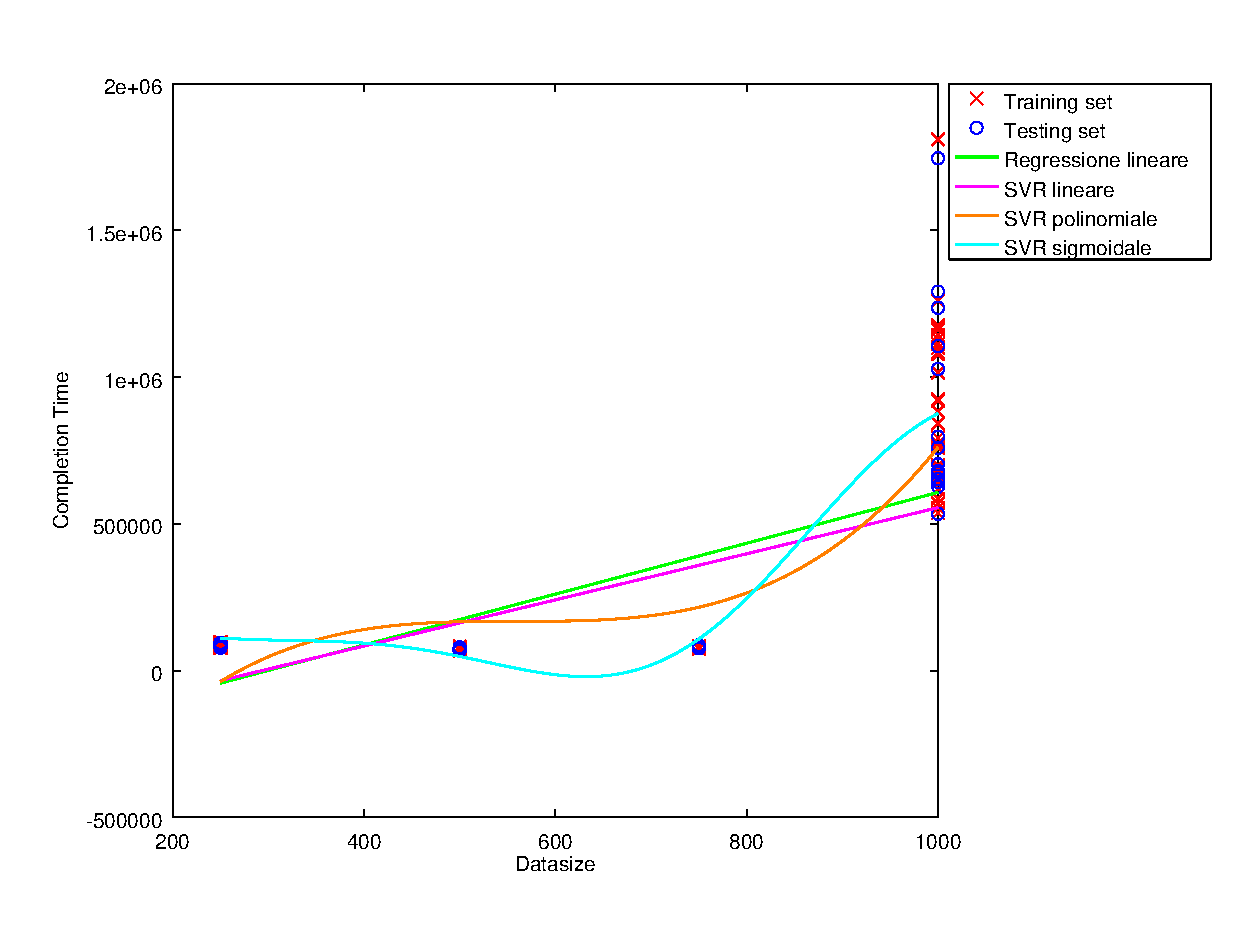
\includegraphics[width=\textwidth]{output/R2_SOLO_DATASIZE/plot_R2.eps}
\caption {Completion time vs Datasize (query R2, solo Datasize)}
\end {figure}

\newpage
\subsection{Query R3 -- solo Datasize}
\begin{table}[bhpt]
	\centering
	\begin{adjustbox}{center}
		\begin{tabular}{c | c M{1cm} M{2.5cm} M{2.5cm} M{1.8cm}}
			Modello & RMSE & R\textsuperscript{2} & Errore assoluto medio & Errore relativo medio \tabularnewline
			\hline
			Regressione lineare & 0.5972 & 0.6072 & 761010 & 1.1226 \\
			SVR lineare & 0.6064 & 0.6101 & 758201 & 0.9973 \\
			SVR polinomiale & 0.6554 & 0.5273 & 785449 & 20.5795 \\
			SVR sigmoidale & 0.6046 & 0.6111 & 758566 & 1.0293 \\
		\end{tabular}
	\end{adjustbox}
	\\
	\caption{Risultati per il test su query R3 (solo Datasize)}
	\label{table_R3_datasize}
\end{table}

\begin {figure}[hbtp]
\centering
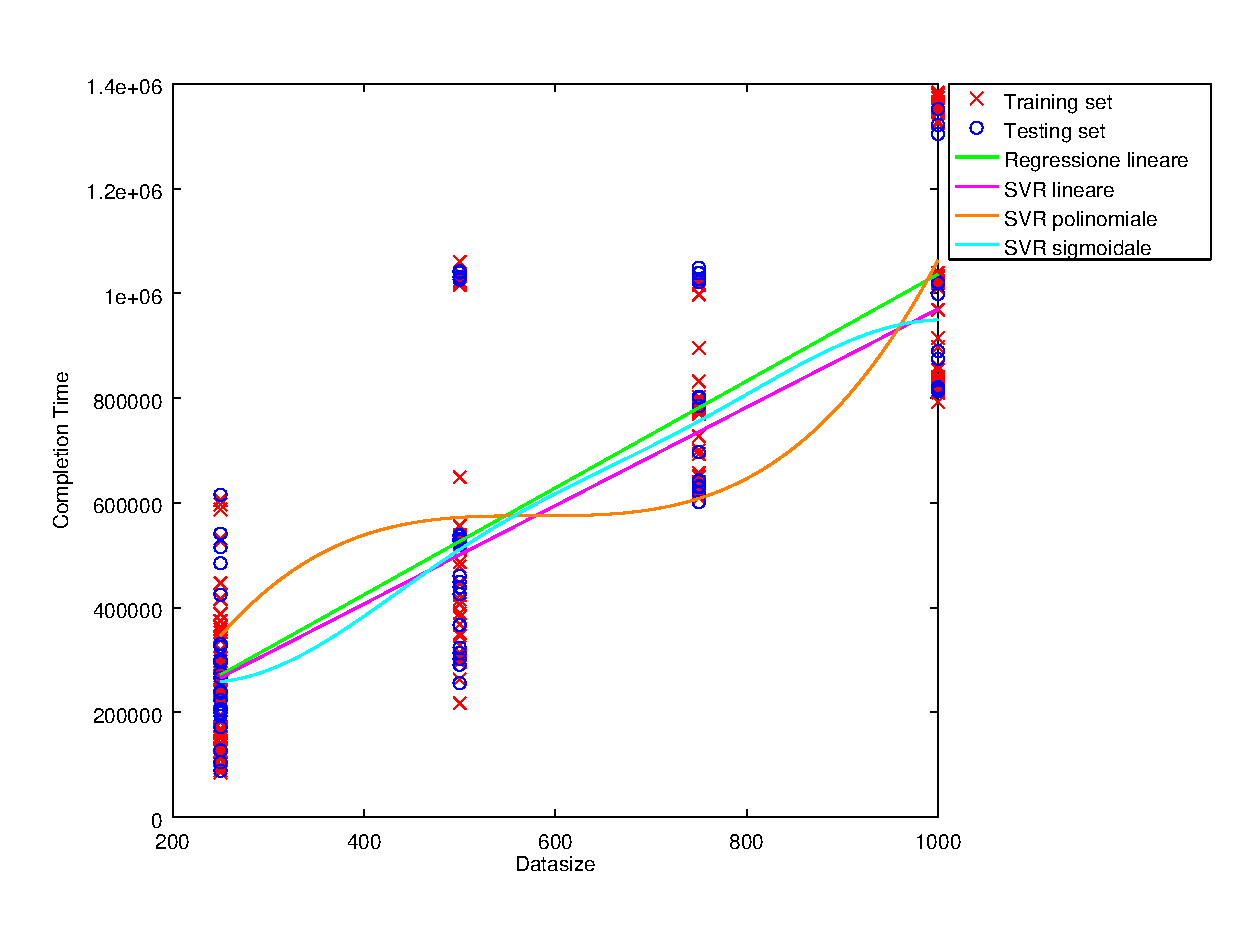
\includegraphics[width=\textwidth]{output/R3_SOLO_DATASIZE/plot_R3.eps}
\caption {Completion time vs Datasize (query R3, solo Datasize)}
\end {figure}

\newpage
\subsection{Query R4 -- solo Datasize}
\begin{table}[bhpt]
	\centering
	\begin{adjustbox}{center}
		\begin{tabular}{c | c M{1cm} M{2.5cm} M{2.5cm} M{1.8cm}}
			Modello & RMSE & R\textsuperscript{2} & Errore assoluto medio & Errore relativo medio \tabularnewline
			\hline
			Regressione lineare & 0.6813 & 0.5673 & 950814 & 1.2418 \\
			SVR lineare & 0.7115 & 0.5755 & 923975 & 1.2164 \\
			SVR polinomiale & 0.5875 & 0.7100 & 892010 & 6.3294 \\
			SVR sigmoidale & 0.5805 & 0.7317 & 844285 & 0.6455 \\
		\end{tabular}
	\end{adjustbox}
	\\
	\caption{Risultati per il test su query R4 (solo Datasize)}
	\label{table_R4_datasize}
\end{table}

\begin {figure}[hbtp]
\centering
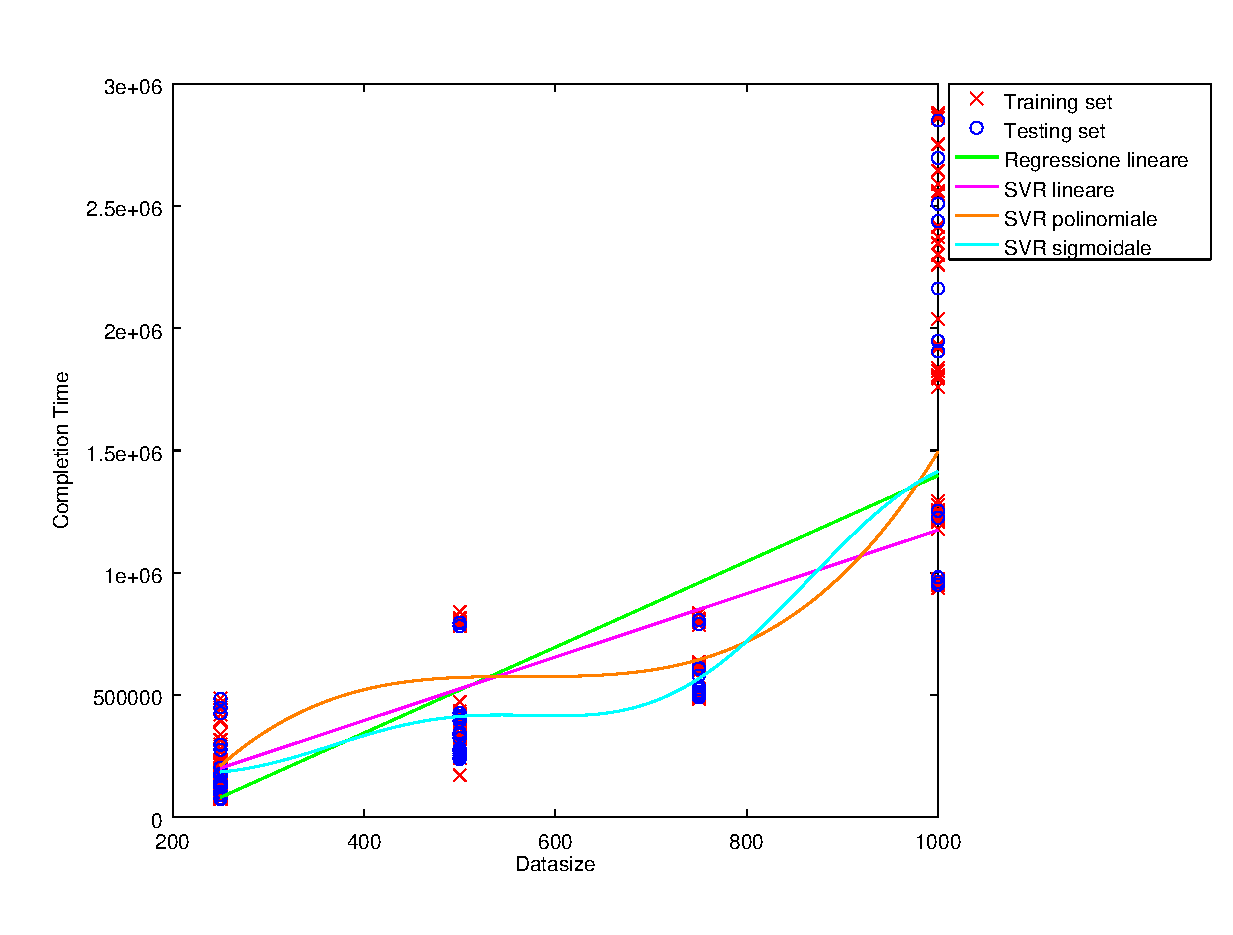
\includegraphics[width=\textwidth]{output/R4_SOLO_DATASIZE/plot_R4.eps}
\caption {Completion time vs Datasize (query R4, solo Datasize)}
\end {figure}

\newpage
\subsection{Query R5 -- solo Datasize}
\begin{table}[bhpt]
	\centering
	\begin{adjustbox}{center}
		\begin{tabular}{c | c M{1cm} M{2.5cm} M{2.5cm} M{1.8cm}}
			Modello & RMSE & R\textsuperscript{2} & Errore assoluto medio & Errore relativo medio \tabularnewline
			\hline
			Regressione lineare & 0.8601 & 0.3309 &  31953 & 2.2261 \\
			SVR lineare & 0.8610 & 0.3377 &  31991 & 2.0043 \\
			SVR polinomiale & 0.7544 & 0.5017 &  31346 & 2.5800 \\
			SVR sigmoidale & 0.6393 & 0.6383 &  29939 & 0.8116 \\
		\end{tabular}
	\end{adjustbox}
	\\
	\caption{Risultati per il test su query R5 (solo Datasize)}
	\label{table_R5_datasize}
\end{table}

\begin {figure}[hbtp]
\centering
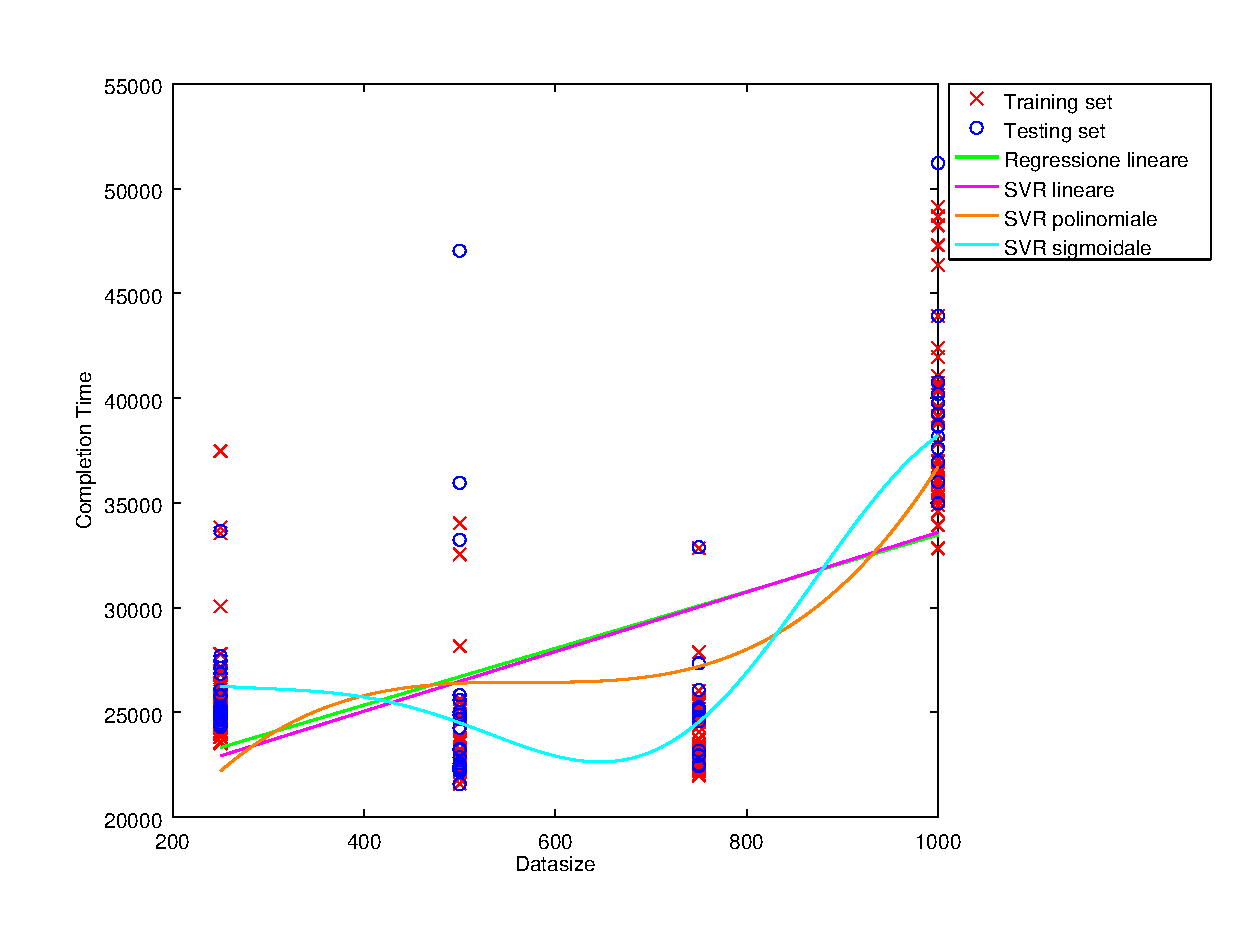
\includegraphics[width=\textwidth]{output/R5_SOLO_DATASIZE/plot_R5.eps}
\caption {Completion time vs Datasize (query R5, solo Datasize)}
\end {figure}


\newpage
\section{Fixed Datasize}

\subsection{Query R1}

\subsubsection{R1 -- Datasize 250}
\begin{table}[bhpt]
	\centering
	\begin{adjustbox}{center}
		\begin{tabular}{c | c M{1.2cm} M{2.5cm} M{2.5cm} M{1.8cm}}
			Modello & RMSE & R\textsuperscript{2} & Errore assoluto medio & Errore relativo medio \tabularnewline
			\hline
			Regressione lineare & 0.1795 & 0.9757 &  56367 & 0.2186 \\
			SVR lineare & 0.1224 & 0.9927 &  55443 & 0.0743 \\
			SVR polinomiale & 1.1146 & 0.8420 &  62456 & 1.2615 \\
			SVR sigmoidale & 0.5988 & 0.7769 &  58614 & 0.5452 \\
		\end{tabular}
	\end{adjustbox}
	\\
	\caption{Risultati per il test su query R1 con datasize 250}
	\label{table_R1_250}
\end{table}

\begin {figure}[hbtp]
\centering
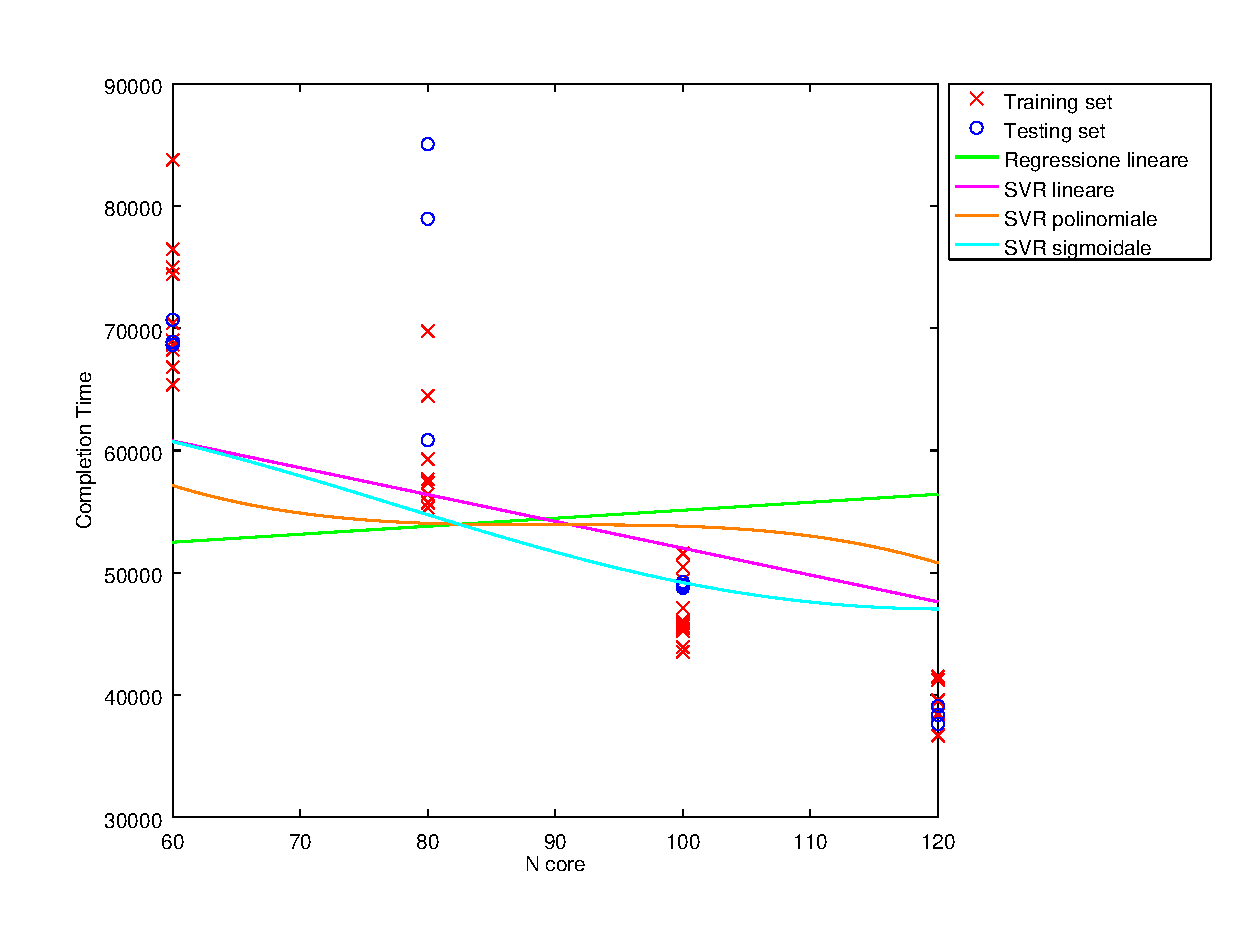
\includegraphics[width=\textwidth]{output/R1_250/plot_R1_250.eps}
\caption {Plot per il test su query R1 con datasize 250}
\end {figure}

\newpage

\newpage
\subsubsection{R1 -- Datasize 500}

\begin{table}[bhpt]
	\centering
	\begin{adjustbox}{center}
		\begin{tabular}{c | c M{1.2cm} M{2.5cm} M{2.5cm} M{1.8cm}}
			Modello & RMSE & R\textsuperscript{2} & Errore assoluto medio & Errore relativo medio \tabularnewline
			\hline
			Regressione lineare & 0.5279 & 0.7681 & 100565 & 1.8233 \\
			SVR lineare & 0.2053 & 0.9737 &  96467 & 0.8926 \\
			SVR polinomiale & 0.8232 & 0.9846 & 105694 & 4.2244 \\
			SVR sigmoidale & 0.6578 & 0.8483 & 101982 & 1.9743 \\
		\end{tabular}
	\end{adjustbox}
	\\
	\caption{Risultati per il test su query R1 con datasize 500}
	\label{table_R1_500}
\end{table}

\begin {figure}[hbt]
\centering
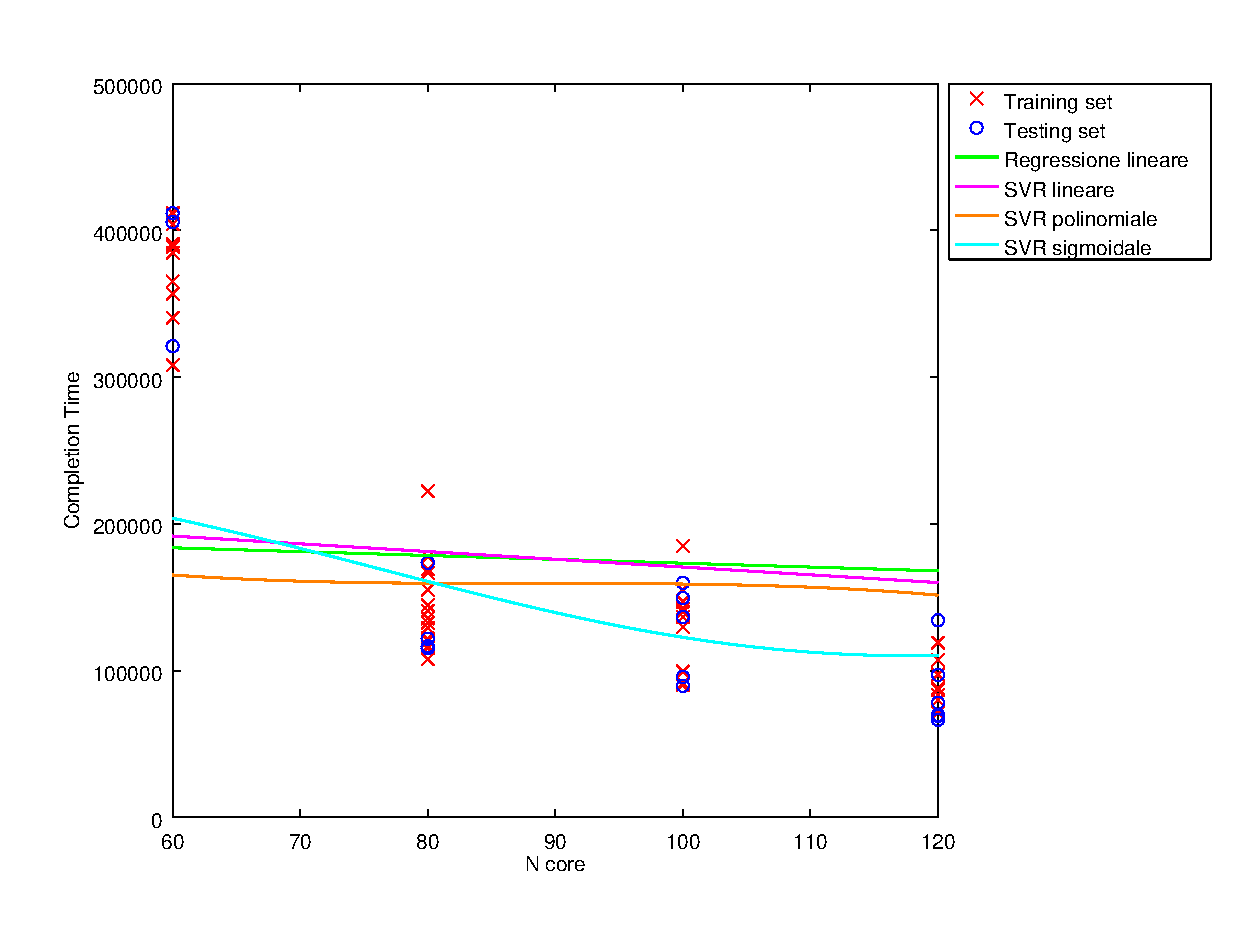
\includegraphics[width=\textwidth]{output/R1_500/plot_R1_500.eps}
\caption {Plot per il test su query R1 con datasize 500}
\end {figure}

\newpage

\newpage
\subsubsection{R1 -- Datasize 750}

\begin{table}[bhpt]
	\centering
	\begin{adjustbox}{center}
		\begin{tabular}{c | c M{1.2cm} M{2.5cm} M{2.5cm} M{1.8cm}}
			Modello & RMSE & R\textsuperscript{2} & Errore assoluto medio & Errore relativo medio \tabularnewline
			\hline
			Regressione lineare & 0.1606 & 0.9676 & 272212 & 1.2198 \\
			SVR lineare & 0.1728 & 0.9644 & 273318 & 2.5279 \\
			SVR polinomiale & 0.3743 & 0.8626 & 285239 & 1.1986 \\
			SVR sigmoidale & 0.1082 & 0.9870 & 269280 & 0.3210 \\
		\end{tabular}
	\end{adjustbox}
	\\
	\caption{Risultati per il test su query R1 con datasize 750}
	\label{table_R1_750}
\end{table}

\begin {figure}[hbtp]
\centering
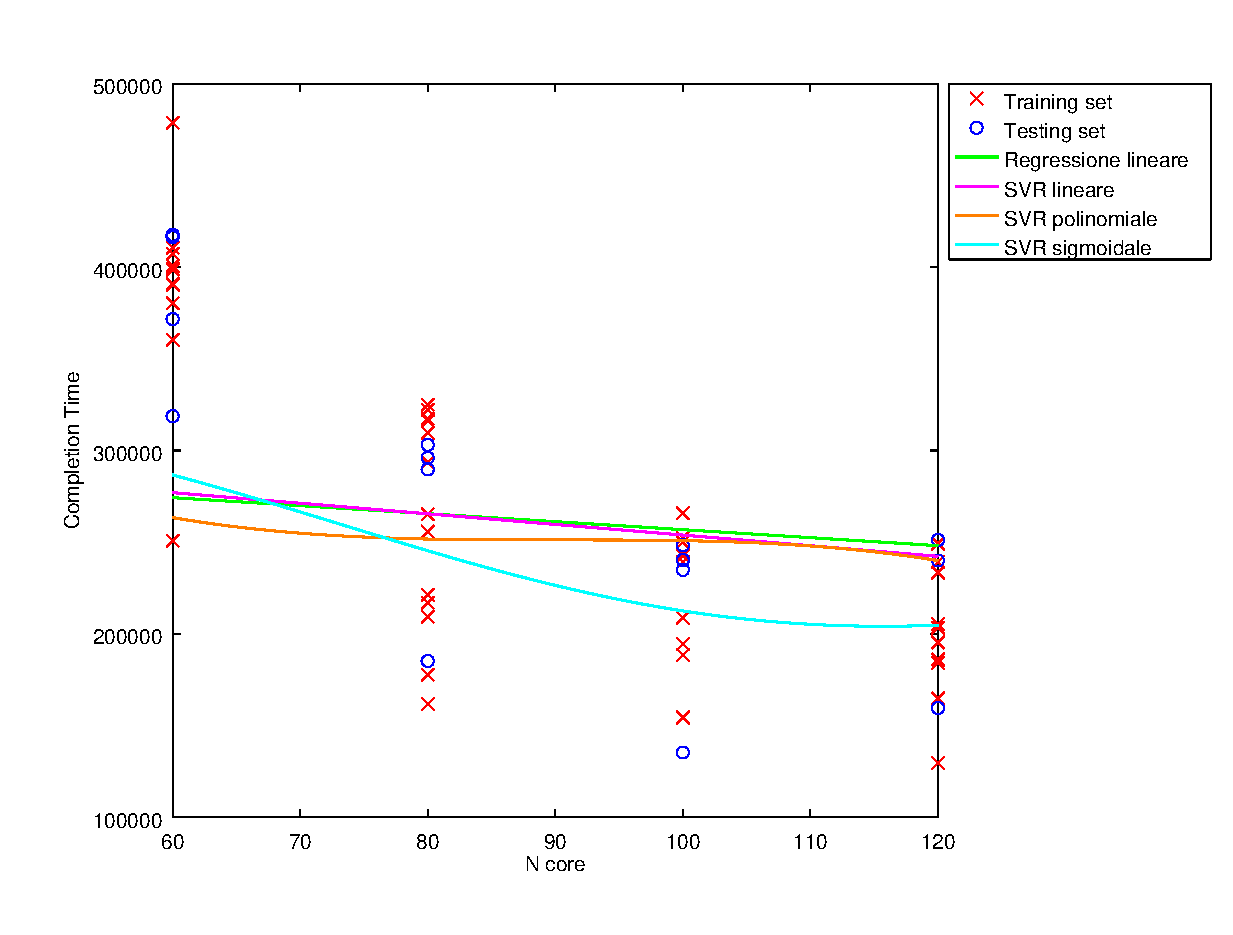
\includegraphics[width=\textwidth]{output/R1_750/plot_R1_750.eps}
\caption {Plot per il test su query R1 con datasize 750}
\end {figure}

\newpage
\newpage
\subsubsection{R1 -- Datasize 1000}
\begin{table}[bhpt]
	\centering
	\begin{adjustbox}{center}
		\begin{tabular}{c | c M{1.2cm} M{2.5cm} M{2.5cm} M{1.8cm}}
			Modello & RMSE & R\textsuperscript{2} & Errore assoluto medio & Errore relativo medio \tabularnewline
			\hline
			Regressione lineare & 0.1019 & 0.9875 & 431805 & 0.3050 \\
			SVR lineare & 0.0943 & 0.9897 & 431858 & 0.3831 \\
			SVR polinomiale & 0.6198 & 0.9260 & 473497 & 3.3538 \\
			SVR sigmoidale & 0.0989 & 0.9920 & 432081 & 0.4642 \\
		\end{tabular}
	\end{adjustbox}
	\\
	\caption{Risultati per il test su query R1 con datasize 1000}
	\label{table_R1_1000}
\end{table}

\begin {figure}[hbtp]
\centering
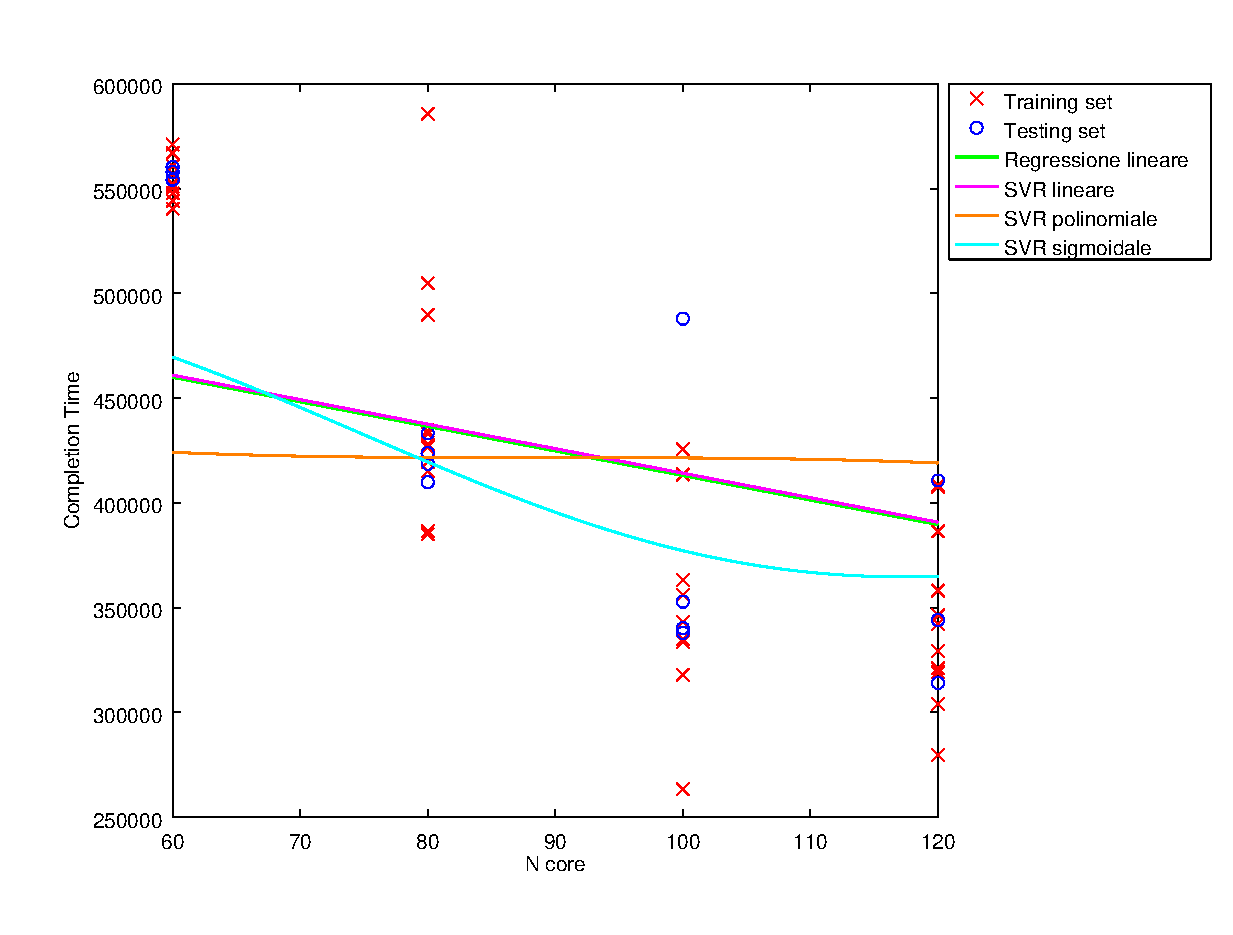
\includegraphics[width=\textwidth]{output/R1_1000/plot_R1_1000.eps}
\caption {Plot per il test su query R1 con datasize 1000}
\end {figure}

\newpage
\subsection{Query R2}

\subsubsection{R2 -- Datasize 250}
\begin{table}[bhpt]
	\centering
	\begin{adjustbox}{center}
		\begin{tabular}{c | c M{1.2cm} M{2.5cm} M{2.5cm} M{1.8cm}}
			Modello & RMSE & R\textsuperscript{2} & Errore assoluto medio & Errore relativo medio \tabularnewline
			\hline
			Regressione lineare & 0.2945 & 0.9300 &  83930 & 1.2256 \\
			SVR lineare & 0.3331 & 0.9107 &  83944 & 1.3726 \\
			SVR polinomiale & 0.5539 & 0.8927 &  84628 & 1.6366 \\
			SVR sigmoidale & 0.4829 & 0.8611 &  84329 & 1.6959 \\
		\end{tabular}
	\end{adjustbox}
	\\
	\caption{Risultati per il test su query R2 con datasize 250}
	\label{table_R2_250}
\end{table}

\begin {figure}[hbtp]
\centering
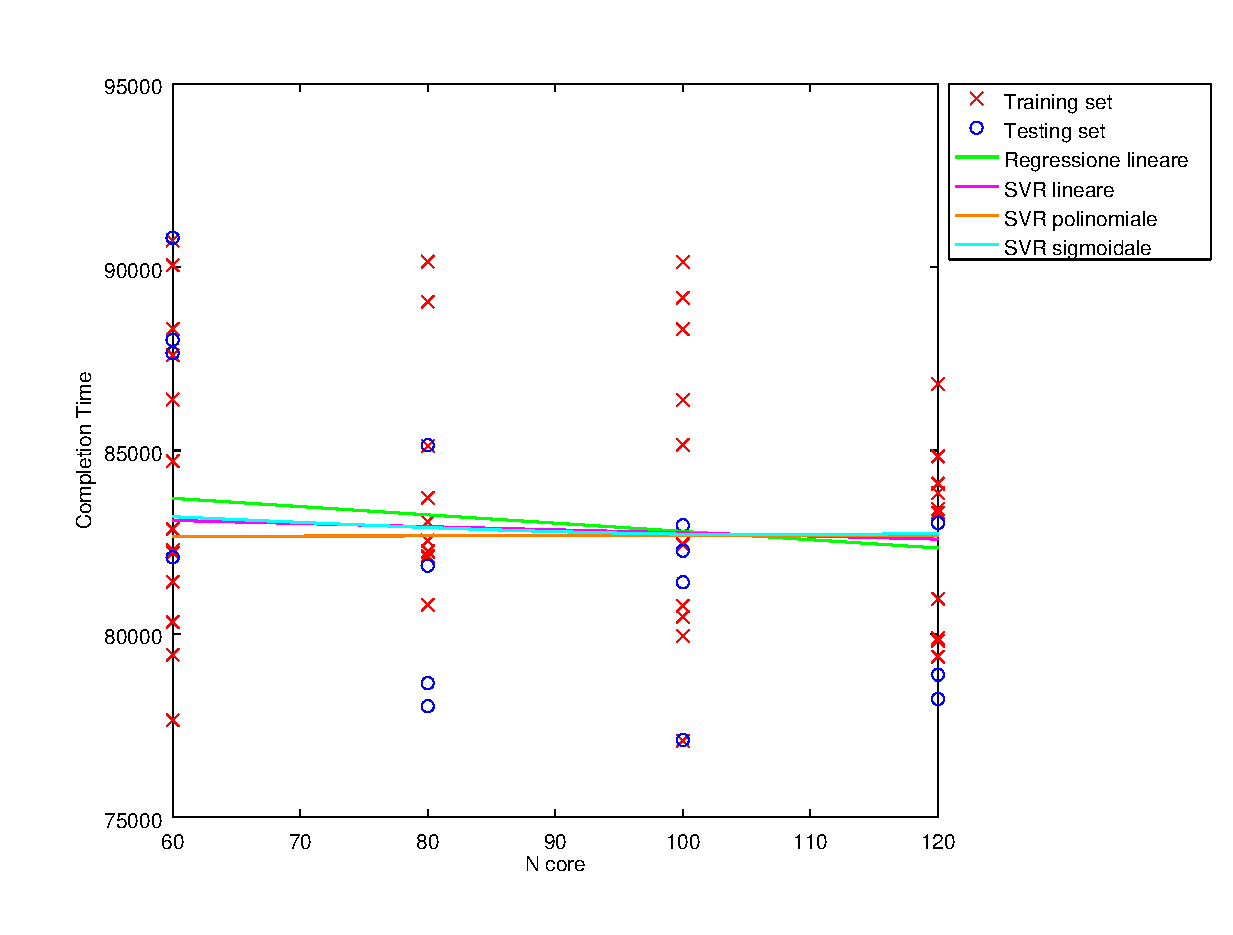
\includegraphics[width=\textwidth]{output/R2_250/plot_R2_250.eps}
\caption {Plot per il test su query R2 con datasize 250}
\end {figure}

\newpage
\subsubsection{R2 -- Datasize 500}
\begin{table}[bhpt]
	\centering
	\begin{adjustbox}{center}
		\begin{tabular}{c | c M{1.2cm} M{2.5cm} M{2.5cm} M{1.8cm}}
			Modello & RMSE & R\textsuperscript{2} & Errore assoluto medio & Errore relativo medio \tabularnewline
			\hline
			Regressione lineare & 0.1810 & 0.9688 &  73280 & 0.4963 \\
			SVR lineare & 0.1800 & 0.9698 &  73280 & 0.4679 \\
			SVR polinomiale & 0.4380 & 0.8193 &  73907 & 2.5618 \\
			SVR sigmoidale & 0.2172 & 0.9578 &  73375 & 0.4690 \\
		\end{tabular}
	\end{adjustbox}
	\\
	\caption{Risultati per il test su query R2 con datasize 500}
	\label{table_R2_500}
\end{table}

\begin {figure}[hbtp]
\centering
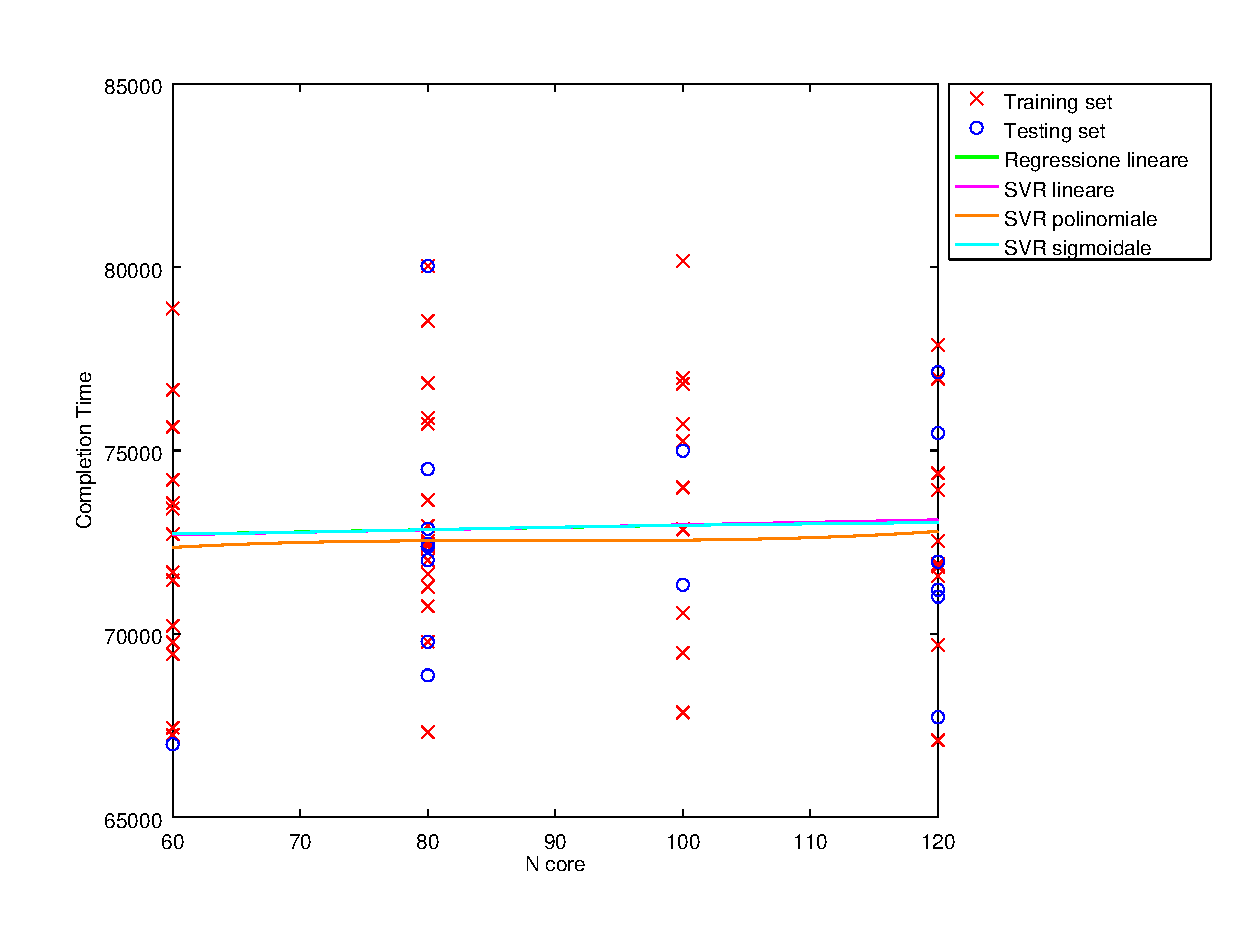
\includegraphics[width=\textwidth]{output/R2_500/plot_R2_500.eps}
\caption {Plot per il test su query R2 con datasize 500}
\end {figure}
\newpage
\subsubsection{R2 -- Datasize 750}
\begin{table}[bhpt]
	\centering
	\begin{adjustbox}{center}
		\begin{tabular}{c | c M{1.2cm} M{2.5cm} M{2.5cm} M{1.8cm}}
			Modello & RMSE & R\textsuperscript{2} & Errore assoluto medio & Errore relativo medio \tabularnewline
			\hline
			Regressione lineare & 0.2172 & 0.9198 &  79129 & 1.6851 \\
			SVR lineare & 0.2177 & 0.9219 &  79103 & 0.5003 \\
			SVR polinomiale & 0.6016 & 0.7222 &  80166 & 9.7460 \\
			SVR sigmoidale & 0.2593 & 0.8958 &  79206 & 0.4017 \\
		\end{tabular}
	\end{adjustbox}
	\\
	\caption{Risultati per il test su query R2 con datasize 750}
	\label{table_R2_750}
\end{table}

\begin {figure}[hbtp]
\centering
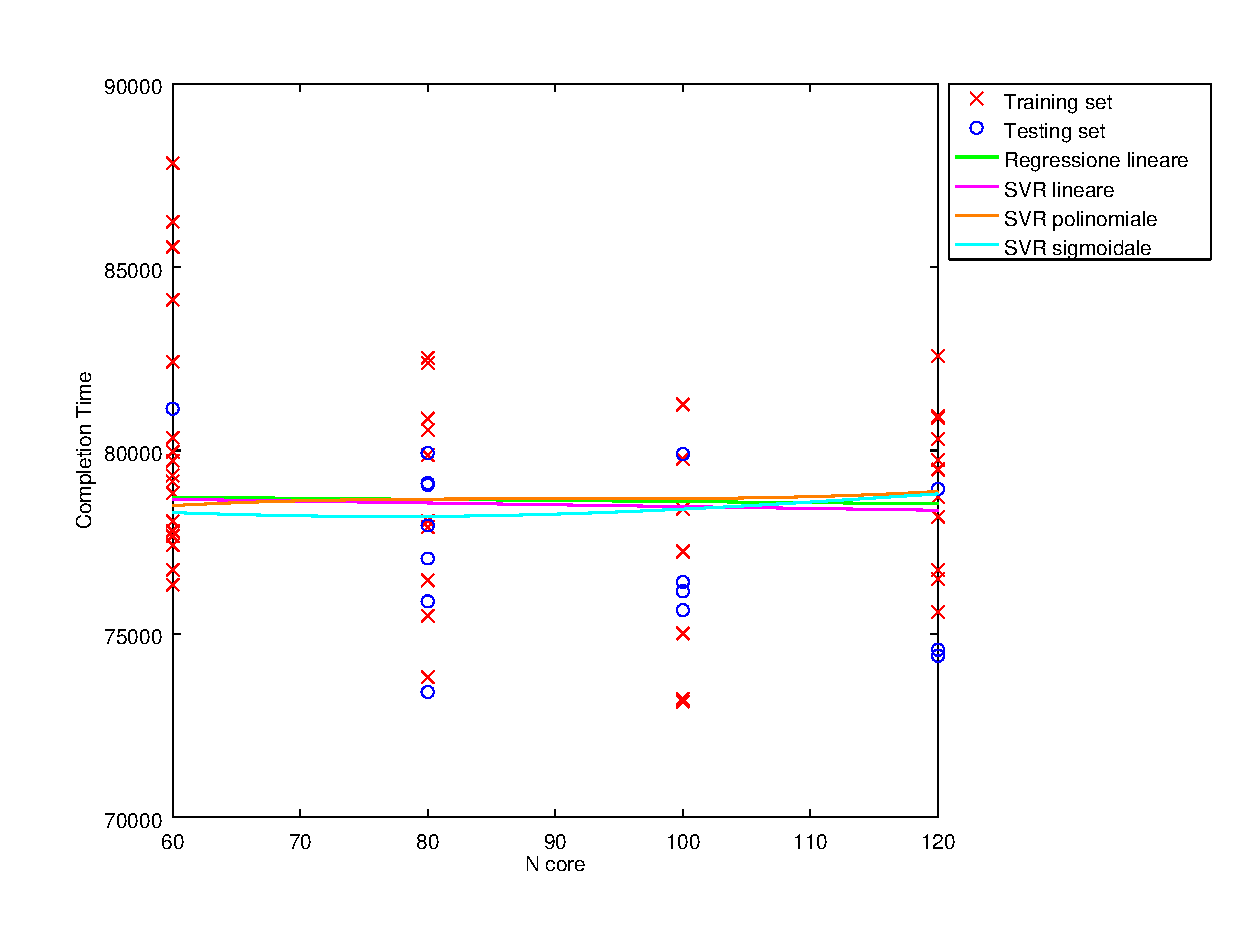
\includegraphics[width=\textwidth]{output/R2_750/plot_R2_750.eps}
\caption {Plot per il test su query R2 con datasize 750}
\end {figure}
\newpage
\subsubsection{R2 -- Datasize 1000}
\begin{table}[bhpt]
	\centering
	\begin{adjustbox}{center}
		\begin{tabular}{c | c M{1.2cm} M{2.5cm} M{2.5cm} M{1.8cm}}
			Modello & RMSE & R\textsuperscript{2} & Errore assoluto medio & Errore relativo medio \tabularnewline
			\hline
			Regressione lineare & 0.6206 & 0.4222 & 1461868 & 1.1535 \\
			SVR lineare & 0.6184 & 0.5211 & 1449291 & 1.5072 \\
			SVR polinomiale & 0.6906 & 0.3466 & 1456778 & 40.6253 \\
			SVR sigmoidale & 0.3406 & 0.8269 & 1289489 & 0.6985 \\
		\end{tabular}
	\end{adjustbox}
	\\
	\caption{Risultati per il test su query R2 con datasize 1000}
	\label{table_R2_1000}
\end{table}

\begin {figure}[hbtp]
\centering
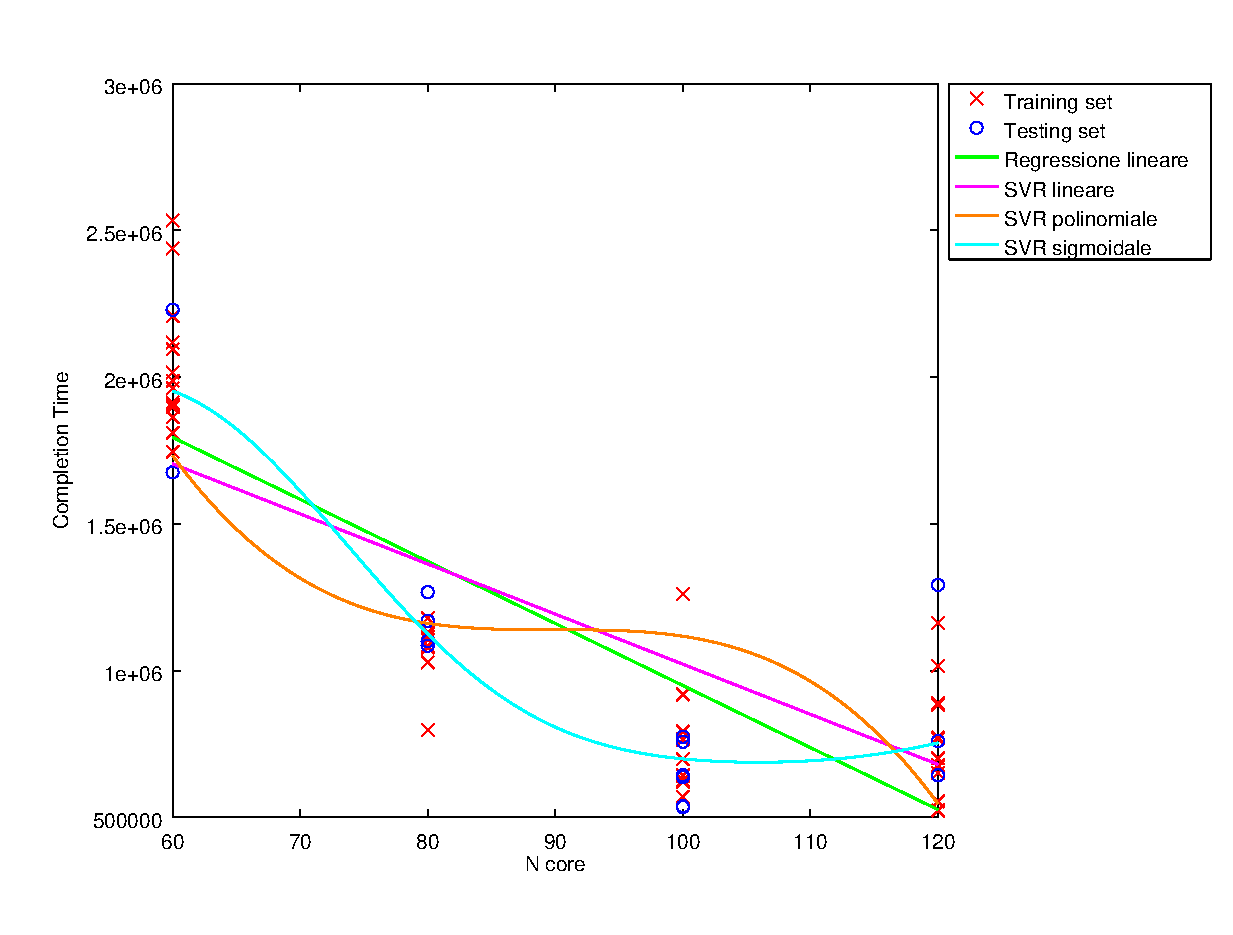
\includegraphics[width=\textwidth]{output/R2_1000/plot_R2_1000.eps}
\caption {Plot per il test su query R2 con datasize 1000}
\end {figure}

\newpage
\subsection{Query R3}

\subsubsection{R3 -- Datasize 250}
\begin{table}[bhpt]
	\centering
	\begin{adjustbox}{center}
		\begin{tabular}{c | c M{1.2cm} M{2.5cm} M{2.5cm} M{1.8cm}}
			Modello & RMSE & R\textsuperscript{2} & Errore assoluto medio & Errore relativo medio \tabularnewline
			\hline
			Regressione lineare & 0.1367 & 0.9728 & 196466 & 1.2421 \\
			SVR lineare & 0.1449 & 0.9716 & 197333 & 1.8465 \\
			SVR polinomiale & 0.2522 & 0.9379 & 203404 & 0.7703 \\
			SVR sigmoidale & 0.3566 & 0.8594 & 208542 & 0.5891 \\
		\end{tabular}
	\end{adjustbox}
	\\
	\caption{Risultati per il test su query R3 con datasize 250}
	\label{table_R3_250}
\end{table}

\begin {figure}[hbtp]
\centering
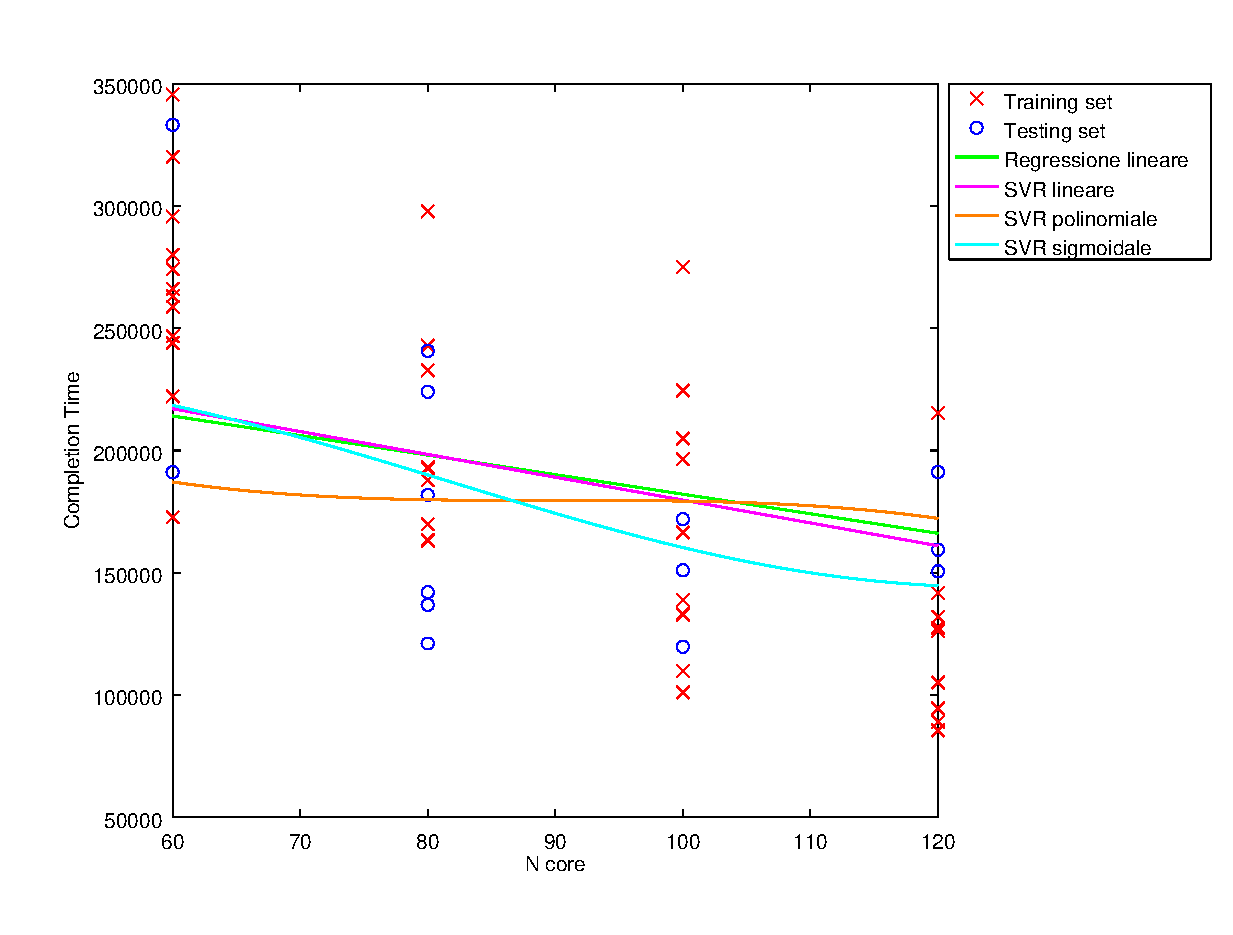
\includegraphics[width=\textwidth]{output/R3_250/plot_R3_250.eps}
\caption {Plot per il test su query R3 con datasize 250}
\end {figure}
\newpage
\subsubsection{R3 -- Datasize 500}
\begin{table}[bhpt]
	\centering
	\begin{adjustbox}{center}
		\begin{tabular}{c | c M{1.2cm} M{2.5cm} M{2.5cm} M{1.8cm}}
			Modello & RMSE & R\textsuperscript{2} & Errore assoluto medio & Errore relativo medio \tabularnewline
			\hline
			Regressione lineare & 0.4296 & 0.7341 & 616021 & 1.6412 \\
			SVR lineare & 0.4369 & 0.7383 & 624688 & 1.1396 \\
			SVR polinomiale & 0.5711 & 0.5604 & 639247 & 0.6813 \\
			SVR sigmoidale & 0.5229 & 0.6132 & 631858 & 159.9640 \\
		\end{tabular}
	\end{adjustbox}
	\\
	\caption{Risultati per il test su query R3 con datasize 500}
	\label{table_R3_500}
\end{table}

\begin {figure}[hbtp]
\centering
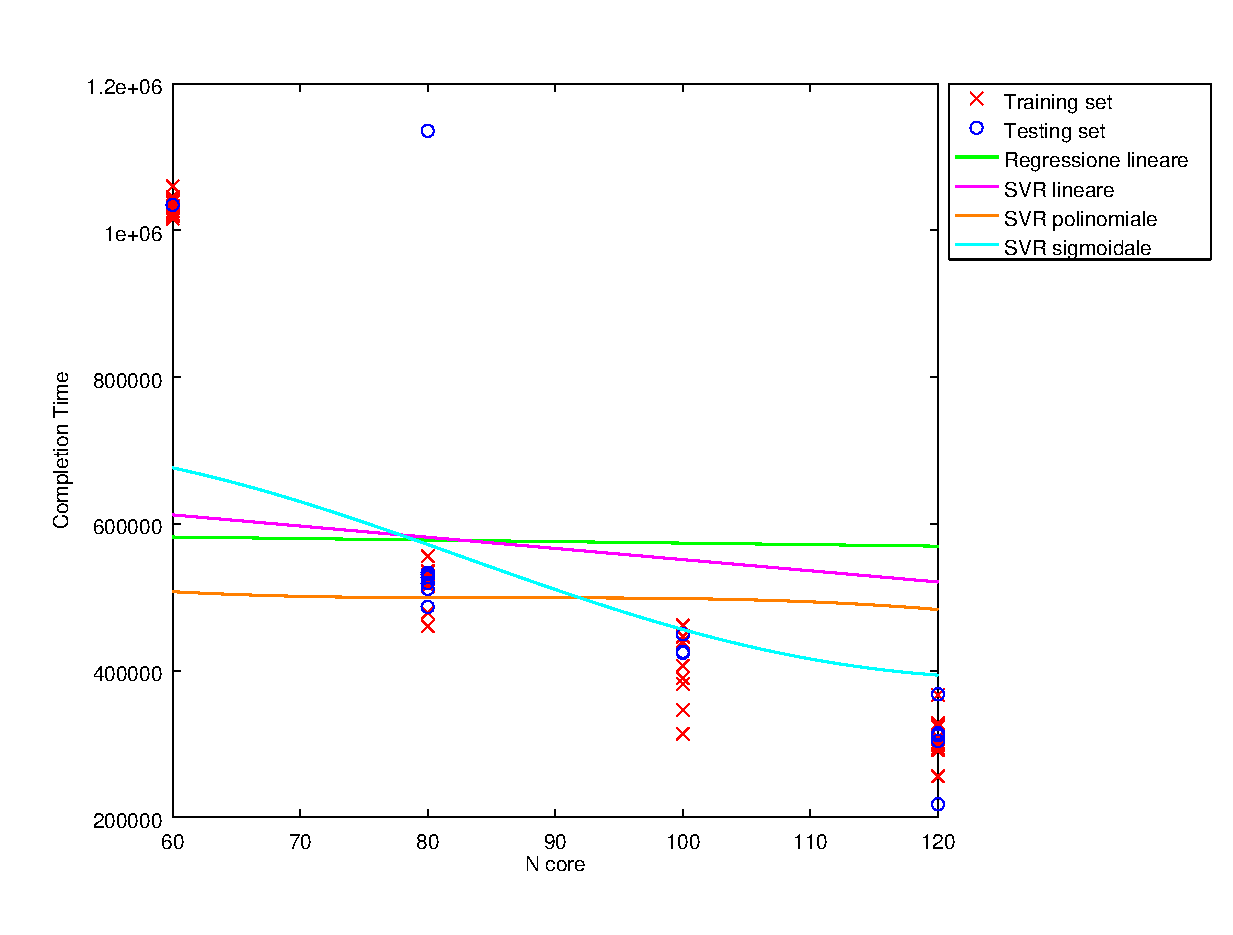
\includegraphics[width=\textwidth]{output/R3_500/plot_R3_500.eps}
\caption {Plot per il test su query R3 con datasize 500}
\end {figure}
\newpage
\subsubsection{R3 -- Datasize 750}
\begin{table}[bhpt]
	\centering
	\begin{adjustbox}{center}
		\begin{tabular}{c | c M{1.2cm} M{2.5cm} M{2.5cm} M{1.8cm}}
			Modello & RMSE & R\textsuperscript{2} & Errore assoluto medio & Errore relativo medio \tabularnewline
			\hline
			Regressione lineare & 0.0336 & 0.9987 & 788712 & 0.1637 \\
			SVR lineare & 0.0701 & 0.9953 & 794619 & 0.2754 \\
			SVR polinomiale & 0.2331 & 0.9436 & 814941 & 0.8557 \\
			SVR sigmoidale & 0.2472 & 0.9388 & 812792 & 1.2858 \\
		\end{tabular}
	\end{adjustbox}
	\\
	\caption{Risultati per il test su query R3 con datasize 750}
	\label{table_R3_750}
\end{table}

\begin {figure}[hbtp]
\centering
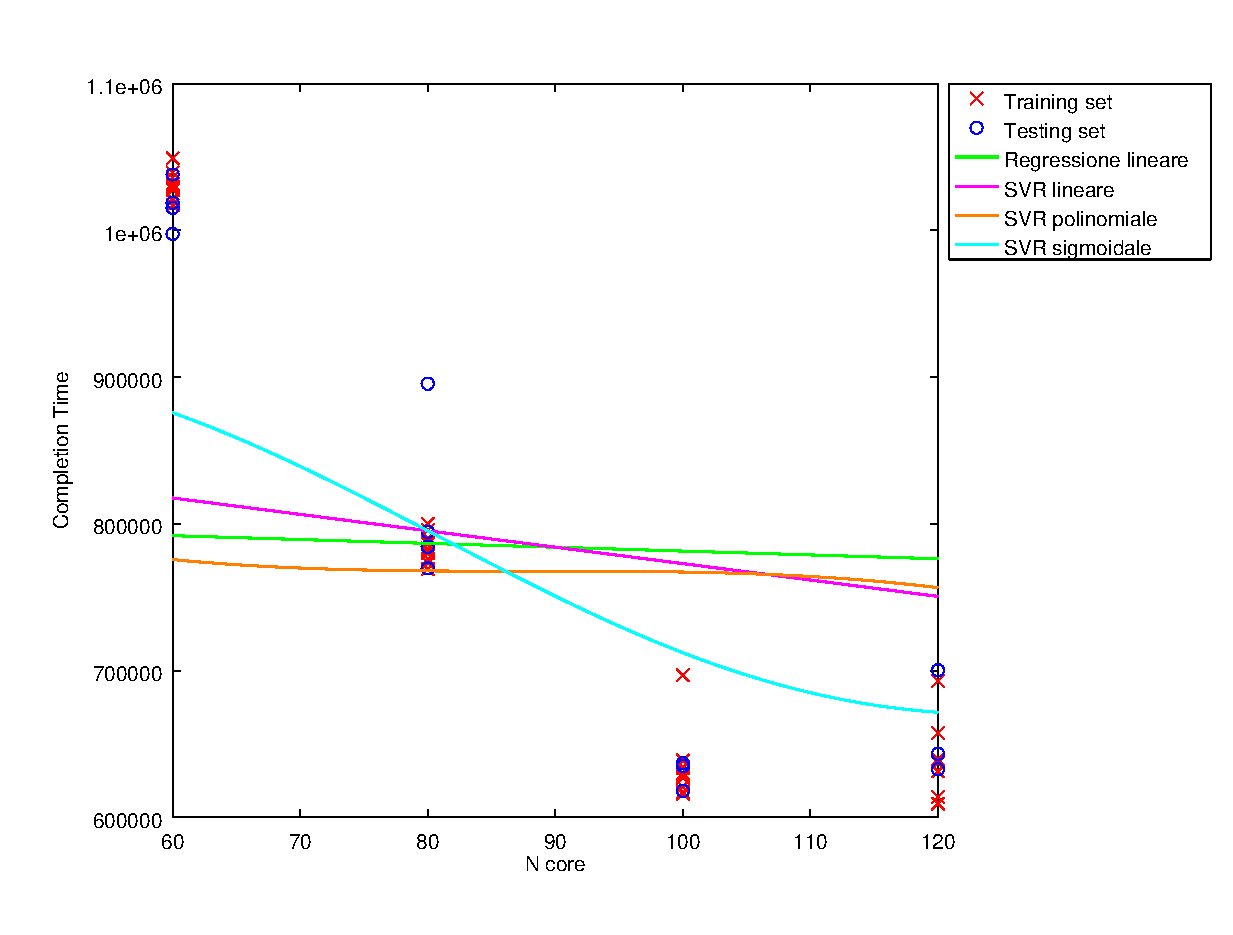
\includegraphics[width=\textwidth]{output/R3_750/plot_R3_750.eps}
\caption {Plot per il test su query R3 con datasize 750}
\end {figure}
\newpage
\subsubsection{R3 -- Datasize 1000}
\begin{table}[bhpt]
	\centering
	\begin{adjustbox}{center}
		\begin{tabular}{c | c M{1.2cm} M{2.5cm} M{2.5cm} M{1.8cm}}
			Modello & RMSE & R\textsuperscript{2} & Errore assoluto medio & Errore relativo medio \tabularnewline
			\hline
			Regressione lineare & 0.0225 & 0.9995 & 1017476 & 0.2029 \\
			SVR lineare & 0.1039 & 0.9916 & 1035277 & 0.3553 \\
			SVR polinomiale & 0.3761 & 0.8810 & 1075249 & 0.4485 \\
			SVR sigmoidale & 0.3269 & 0.9232 & 1063963 & 0.5882 \\
		\end{tabular}
	\end{adjustbox}
	\\
	\caption{Risultati per il test su query R3 con datasize 1000}
	\label{table_R3_1000}
\end{table}

\begin {figure}[hbtp]
\centering
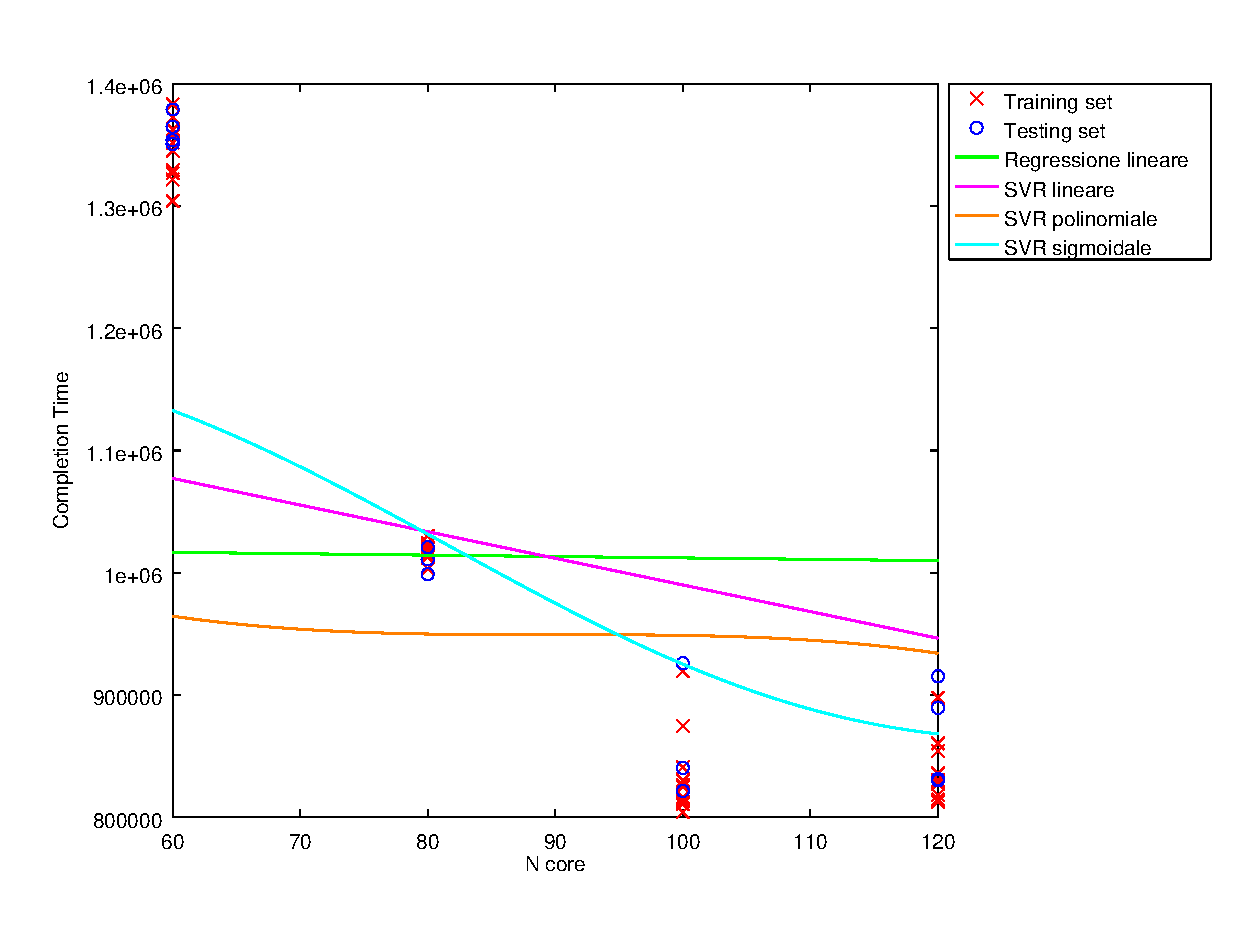
\includegraphics[width=\textwidth]{output/R3_1000/plot_R3_1000.eps}
\caption {Plot per il test su query R3 con datasize 1000}
\end {figure}

\newpage
\subsection{Query R4}

\subsubsection{R4 -- Datasize 250}
\begin{table}[bhpt]
	\centering
	\begin{adjustbox}{center}
		\begin{tabular}{c | c M{1.2cm} M{2.5cm} M{2.5cm} M{1.8cm}}
			Modello & RMSE & R\textsuperscript{2} & Errore assoluto medio & Errore relativo medio \tabularnewline
			\hline
			Regressione lineare & 0.1366 & 0.9770 & 163760 & 0.2719 \\
			SVR lineare & 0.1426 & 0.9758 & 164053 & 0.2698 \\
			SVR polinomiale & 0.3301 & 0.8880 & 172301 & 5.7912 \\
			SVR sigmoidale & 0.2201 & 0.9539 & 164805 & 0.3189 \\
		\end{tabular}
	\end{adjustbox}
	\\
	\caption{Risultati per il test su query R4 con datasize 250}
	\label{table_R4_250}
\end{table}

\begin {figure}[hbtp]
\centering
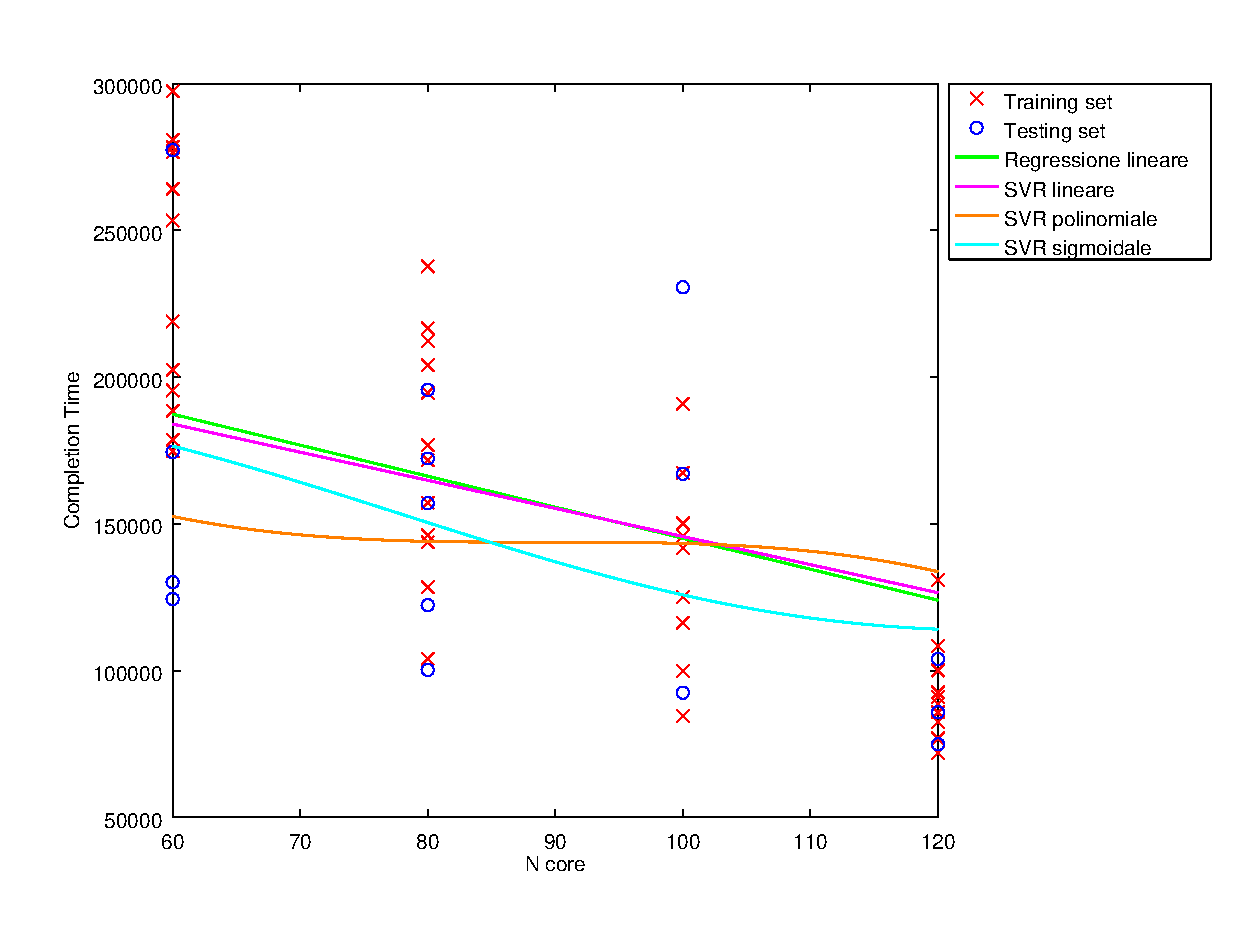
\includegraphics[width=\textwidth]{output/R4_250/plot_R4_250.eps}
\caption {Plot per il test su query R4 con datasize 250}
\end {figure}
\newpage
\subsubsection{R4 -- Datasize 500}
\begin{table}[bhpt]
	\centering
	\begin{adjustbox}{center}
		\begin{tabular}{c | c M{1.2cm} M{2.5cm} M{2.5cm} M{1.8cm}}
			Modello & RMSE & R\textsuperscript{2} & Errore assoluto medio & Errore relativo medio \tabularnewline
			\hline
			Regressione lineare & 0.4873 & 0.7455 & 481376 & 1.6211 \\
			SVR lineare & 0.4836 & 0.7583 & 488122 & 3.2325 \\
			SVR polinomiale & 0.5518 & 0.6898 & 511493 & 2.2149 \\
			SVR sigmoidale & 0.5141 & 0.7193 & 494295 & 1.1828 \\
		\end{tabular}
	\end{adjustbox}
	\\
	\caption{Risultati per il test su query R4 con datasize 500}
	\label{table_R4_500}
\end{table}

\begin {figure}[hbtp]
\centering
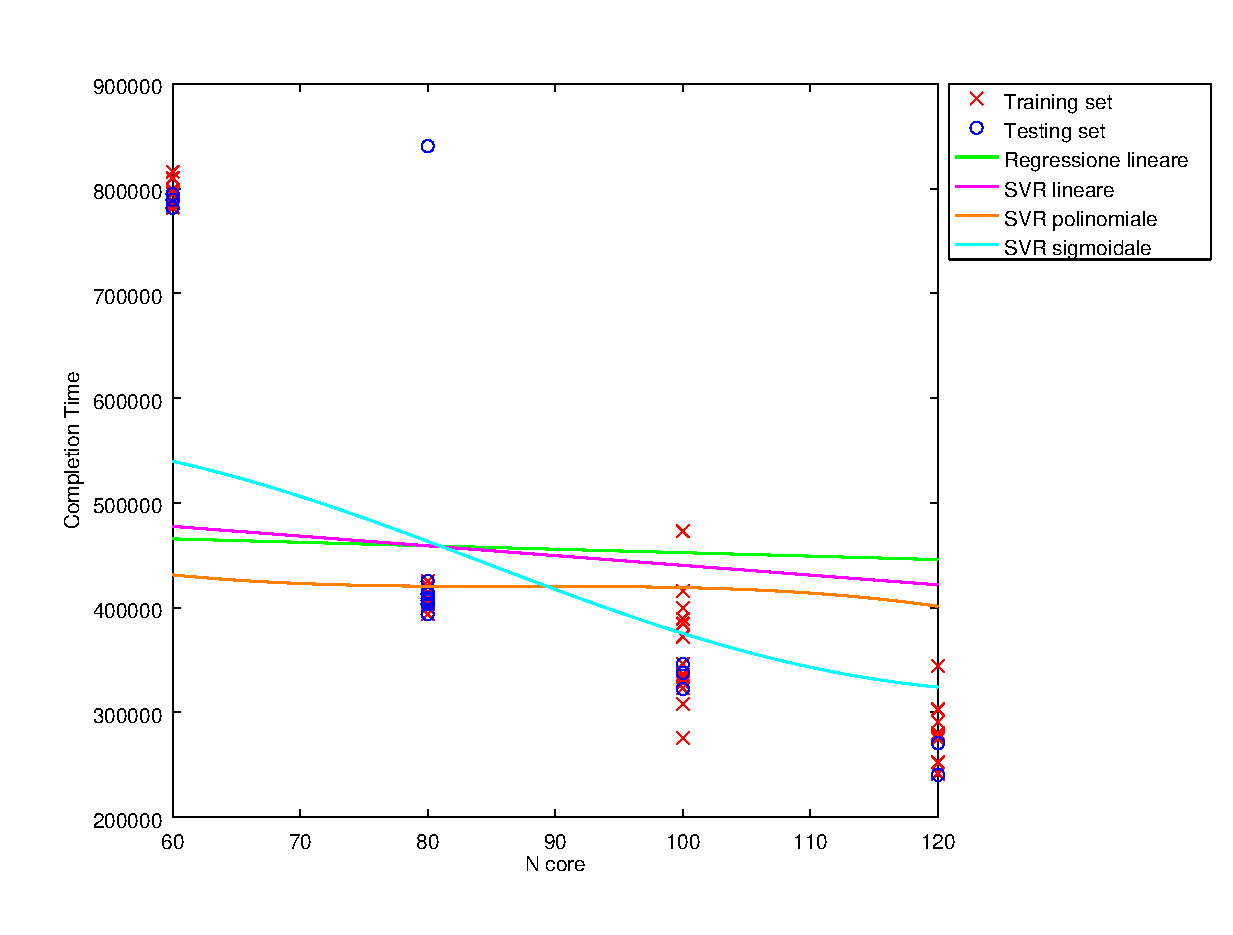
\includegraphics[width=\textwidth]{output/R4_500/plot_R4_500.eps}
\caption {Plot per il test su query R4 con datasize 500}
\end {figure}
\newpage
\subsubsection{R4 -- Datasize 750}
\begin{table}[bhpt]
	\centering
	\begin{adjustbox}{center}
		\begin{tabular}{c | c M{1.2cm} M{2.5cm} M{2.5cm} M{1.8cm}}
			Modello & RMSE & R\textsuperscript{2} & Errore assoluto medio & Errore relativo medio \tabularnewline
			\hline
			Regressione lineare & 0.0248 & 0.9993 & 620160 & 0.1281 \\
			SVR lineare & 0.0816 & 0.9936 & 627111 & 0.7623 \\
			SVR polinomiale & 0.3360 & 0.9021 & 649491 & 0.7968 \\
			SVR sigmoidale & 0.1712 & 0.9722 & 632970 & 0.4241 \\
		\end{tabular}
	\end{adjustbox}
	\\
	\caption{Risultati per il test su query R4 con datasize 750}
	\label{table_R4_750}
\end{table}

\begin {figure}[hbtp]
\centering
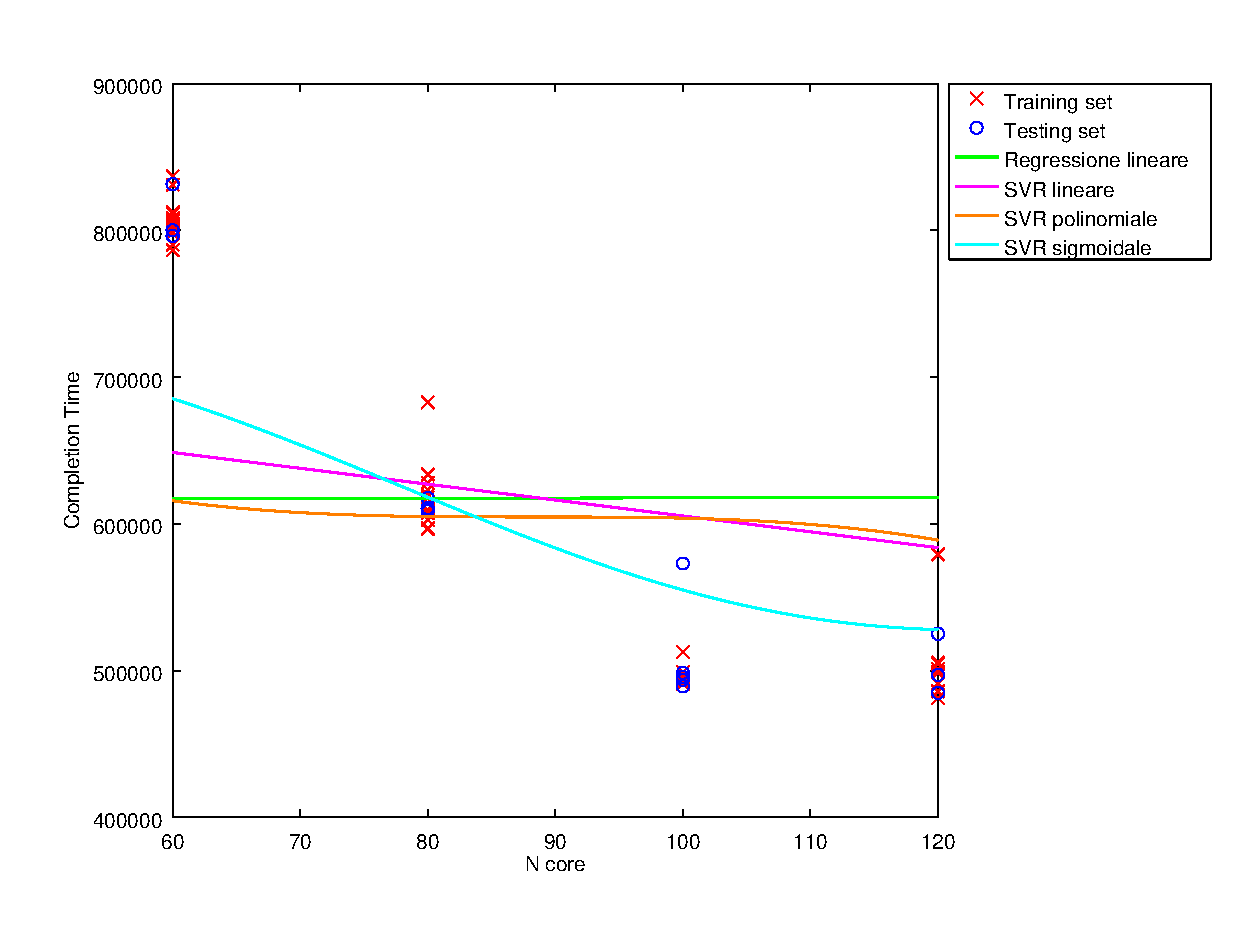
\includegraphics[width=\textwidth]{output/R4_750/plot_R4_750.eps}
\caption {Plot per il test su query R4 con datasize 750}
\end {figure}
\newpage
\subsubsection{R4 -- Datasize 1000}

\begin{table}[bhpt]
	\centering
	\begin{adjustbox}{center}
		\begin{tabular}{c | c M{1.2cm} M{2.5cm} M{2.5cm} M{1.8cm}}
			Modello & RMSE & R\textsuperscript{2} & Errore assoluto medio & Errore relativo medio \tabularnewline
			\hline
			Regressione lineare & 0.1125 & 0.9886 & 1937660 & 0.3304 \\
			SVR lineare & 0.1180 & 0.9883 & 1933919 & 0.8125 \\
			SVR polinomiale & 0.6788 & 0.8269 & 2236602 & 4.5318 \\
			SVR sigmoidale & 0.2119 & 0.9649 & 2001964 & 0.2980 \\
		\end{tabular}
	\end{adjustbox}
	\\
	\caption{Risultati per il test su query R4 con datasize 1000}
	\label{table_R4_1000}
\end{table}

\begin {figure}[hbtp]
\centering
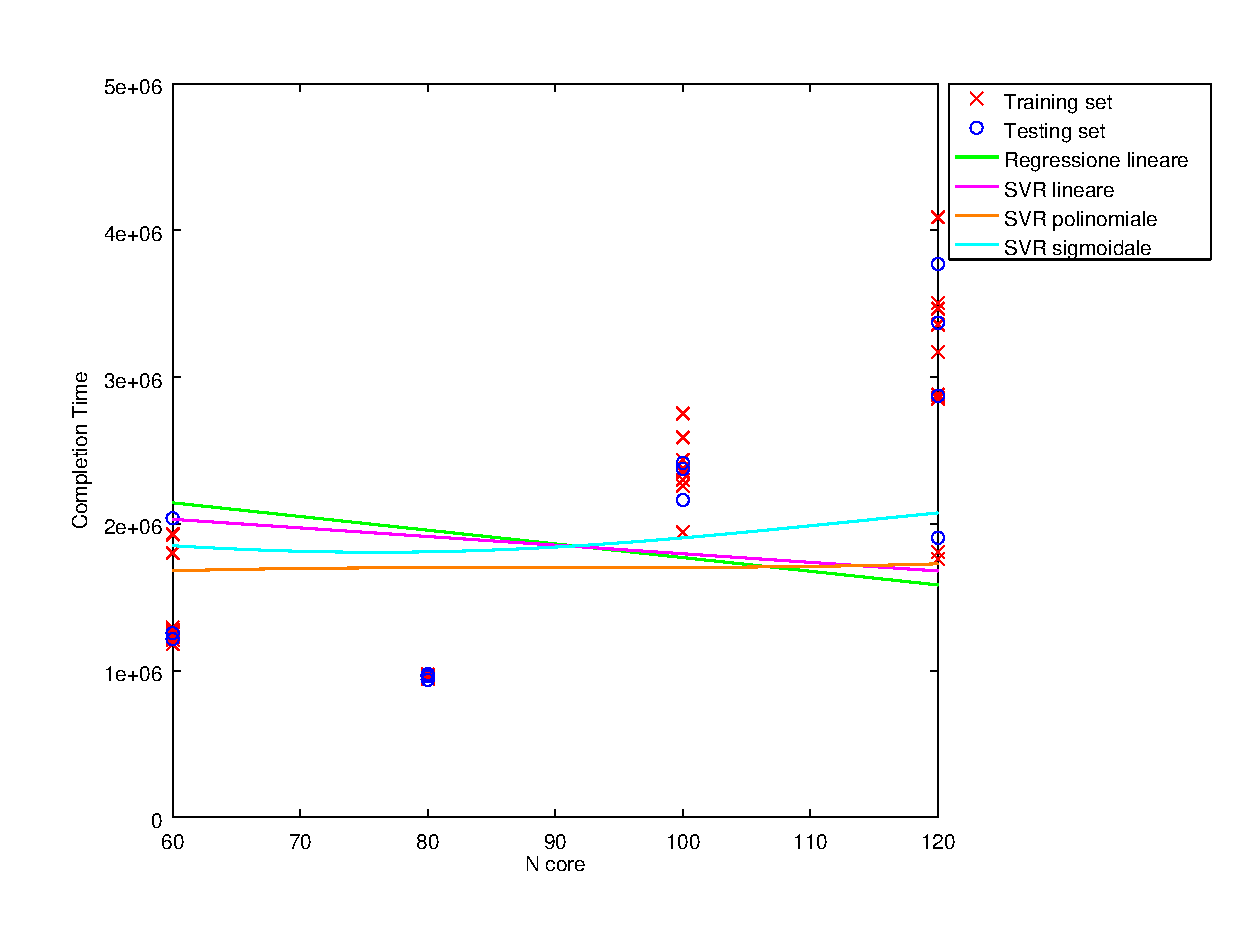
\includegraphics[width=\textwidth]{output/R4_1000/plot_R4_1000.eps}
\caption {Plot per il test su query R4 con datasize 1000}
\end {figure}

\newpage
\subsection{Query R5}

\subsubsection{R5 -- Datasize 250}
\begin{table}[bhpt]
	\centering
	\begin{adjustbox}{center}
		\begin{tabular}{c | c M{1.2cm} M{2.5cm} M{2.5cm} M{1.8cm}}
			Modello & RMSE & R\textsuperscript{2} & Errore assoluto medio & Errore relativo medio \tabularnewline
			\hline
			Regressione lineare & 0.7396 & 0.5197 &  25756 & 1.4684 \\
			SVR lineare & 0.7232 & 0.7663 &  25801 & 2.5330 \\
			SVR polinomiale & 1.2789 & 0.1267 &  26188 & 5.1048 \\
			SVR sigmoidale & 0.9120 & 0.5705 &  25976 & 7.3267 \\
		\end{tabular}
	\end{adjustbox}
	\\
	\caption{Risultati per il test su query R5 con datasize 250}
	\label{table_R5_250}
\end{table}

\begin {figure}[hbtp]
\centering
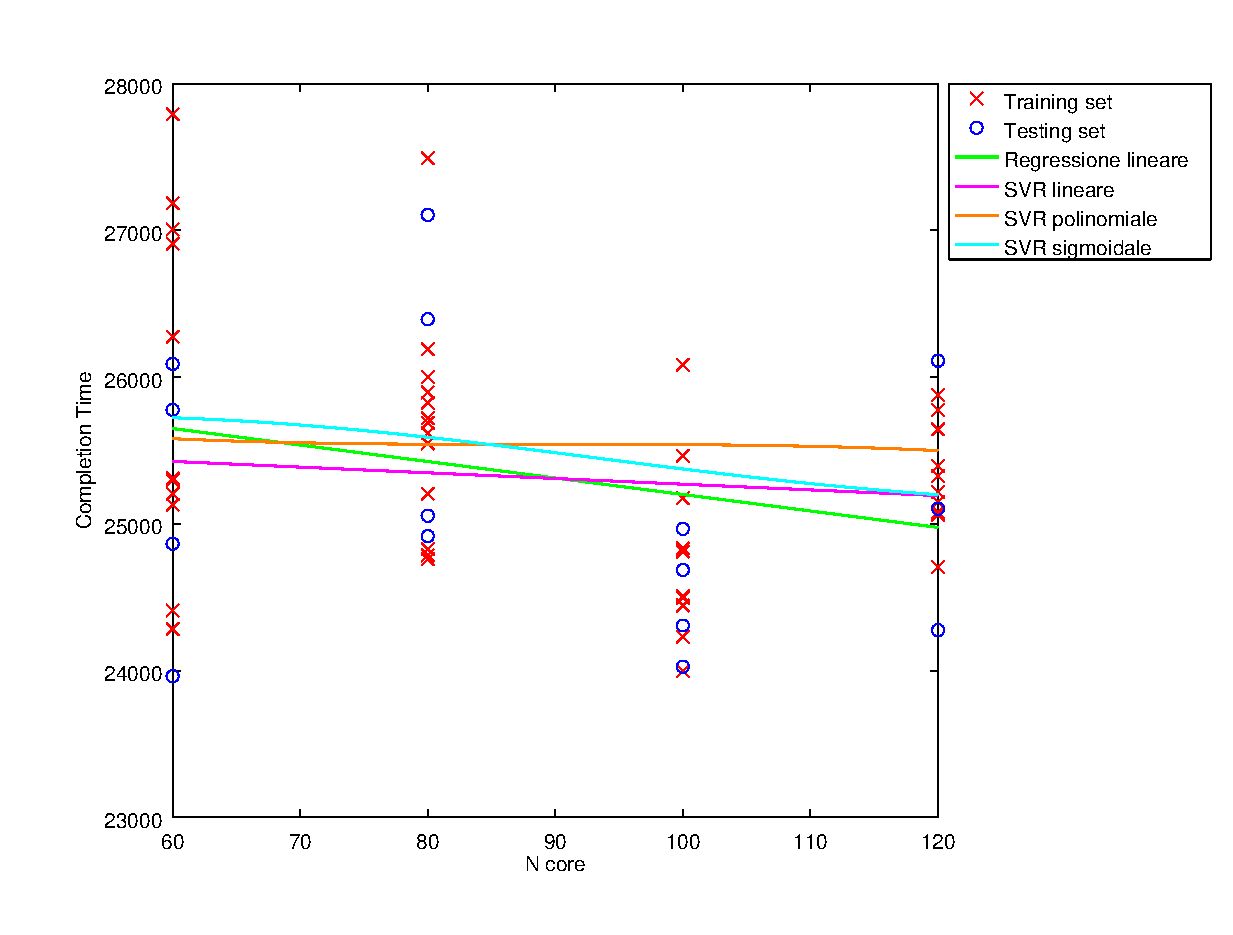
\includegraphics[width=\textwidth]{output/R5_250/plot_R5_250.eps}
\caption {Plot per il test su query R5 con datasize 250}
\end {figure}
\newpage
\subsubsection{R5 -- Datasize 500}
\begin{table}[bhpt]
	\centering
	\begin{adjustbox}{center}
		\begin{tabular}{c | c M{1.2cm} M{2.5cm} M{2.5cm} M{1.8cm}}
			Modello & RMSE & R\textsuperscript{2} & Errore assoluto medio & Errore relativo medio \tabularnewline
			\hline
			Regressione lineare & 0.5126 & 0.5127 &  24308 & 1.2420 \\
			SVR lineare & 0.1699 & 0.9472 &  23876 & 1.5843 \\
			SVR polinomiale & 1.0731 & 0.6518 &  24596 & 1.3832 \\
			SVR sigmoidale & 0.5384 & 0.4989 &  24179 & 0.9291 \\
		\end{tabular}
	\end{adjustbox}
	\\
	\caption{Risultati per il test su query R5 con datasize 500}
	\label{table_R5_500}
\end{table}

\begin {figure}[hbtp]
\centering
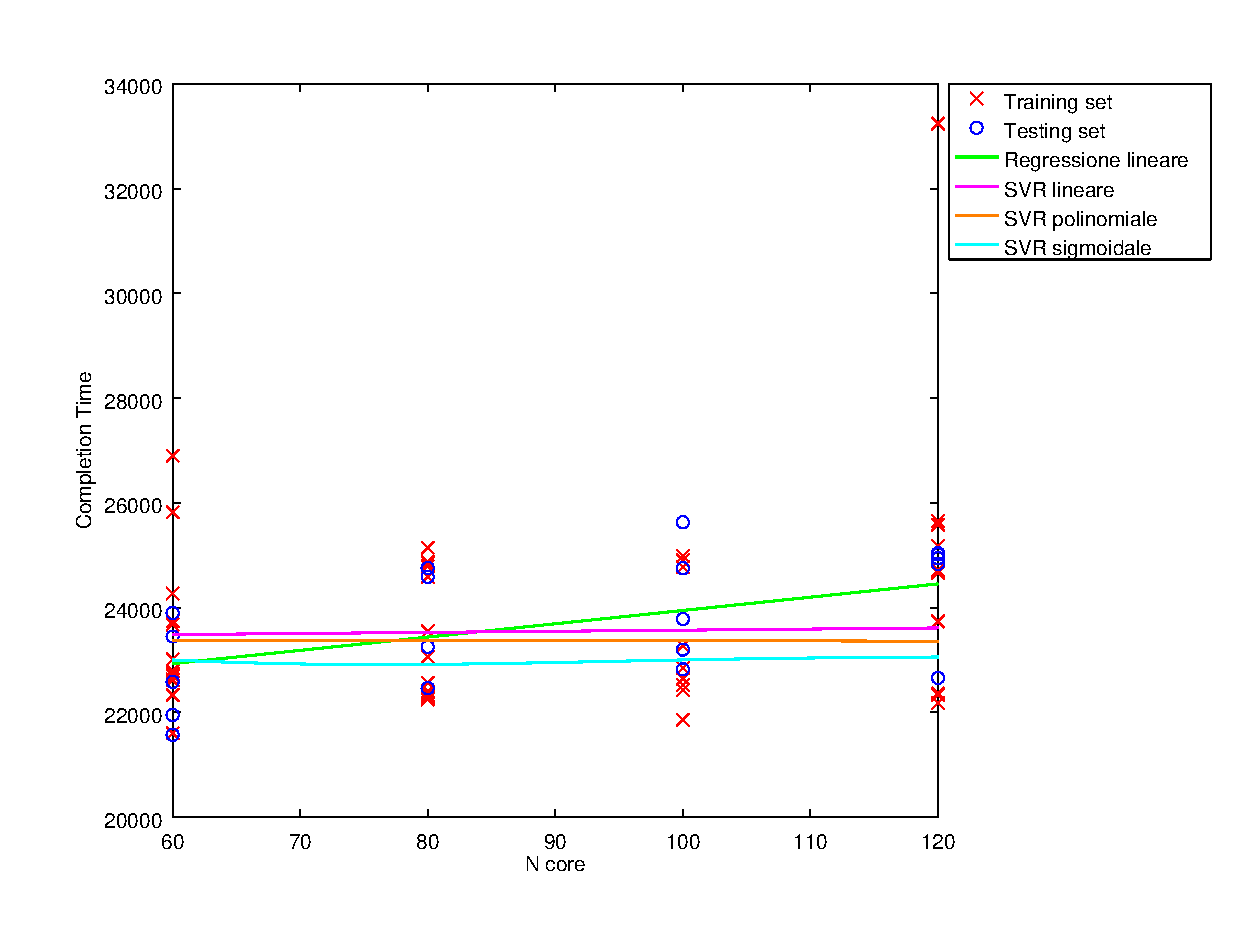
\includegraphics[width=\textwidth]{output/R5_500/plot_R5_500.eps}
\caption {Plot per il test su query R5 con datasize 500}
\end {figure}
\newpage
\subsubsection{R5 -- Datasize 750}
\begin{table}[bhpt]
	\centering
	\begin{adjustbox}{center}
		\begin{tabular}{c | c M{1.2cm} M{2.5cm} M{2.5cm} M{1.8cm}}
			Modello & RMSE & R\textsuperscript{2} & Errore assoluto medio & Errore relativo medio \tabularnewline
			\hline
			Regressione lineare & 0.9679 & 0.1647 &  24739 & 1.1966 \\
			SVR lineare & 0.9723 & 0.2832 &  24696 & 1.3507 \\
			SVR polinomiale & 1.1618 & 0.0687 &  24899 & 2.0287 \\
			SVR sigmoidale & 1.0636 & 0.1689 &  24810 & 1.5607 \\
		\end{tabular}
	\end{adjustbox}
	\\
	\caption{Risultati per il test su query R5 con datasize 750}
	\label{table_R5_750}
\end{table}

\begin {figure}[hbtp]
\centering
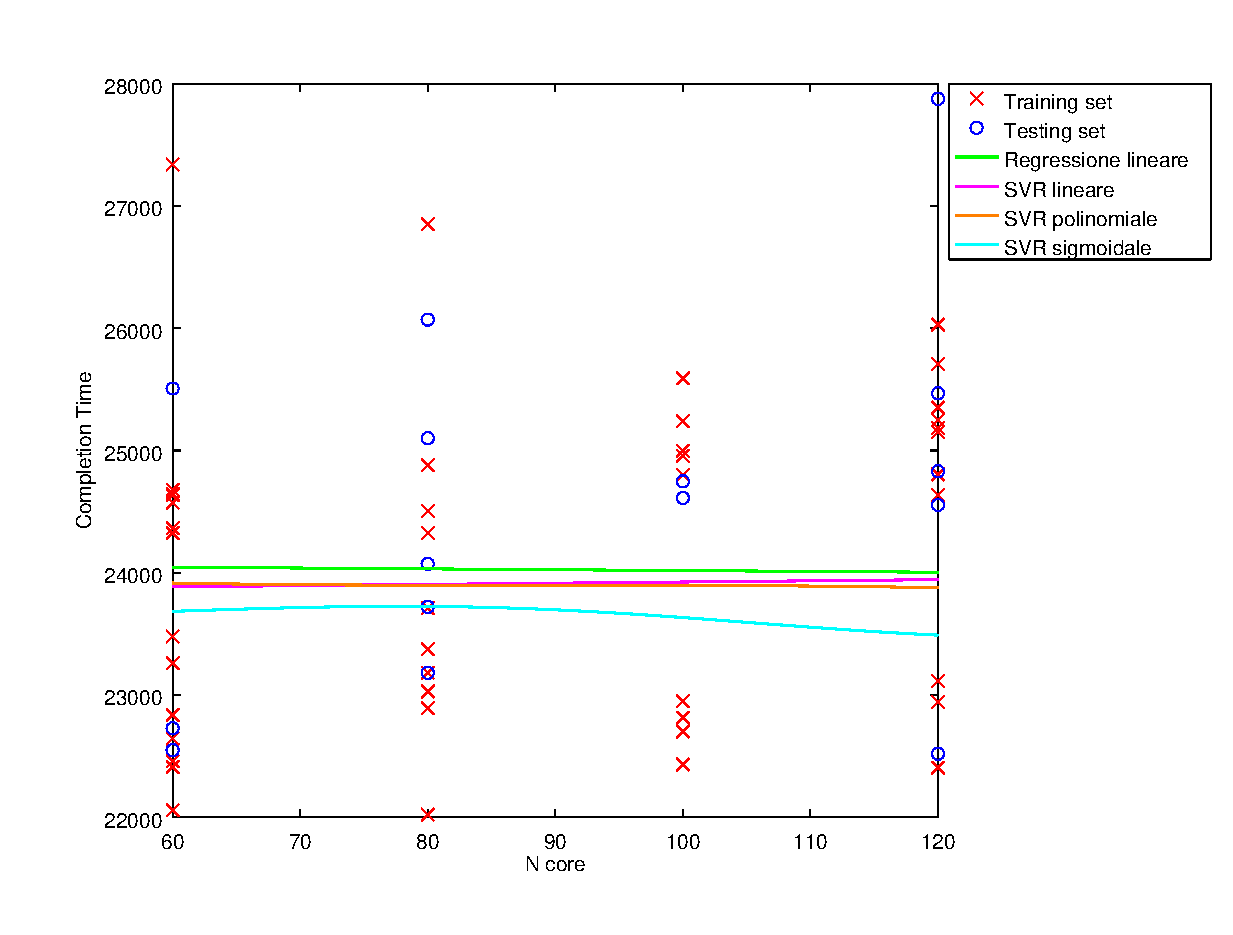
\includegraphics[width=\textwidth]{output/R5_750/plot_R5_750.eps}
\caption {Plot per il test su query R5 con datasize 750}
\end {figure}
\newpage
\subsubsection{R5 -- Datasize 1000}
\begin{table}[bhpt]
	\centering
	\begin{adjustbox}{center}
		\begin{tabular}{c | c M{1.2cm} M{2.5cm} M{2.5cm} M{1.8cm}}
			Modello & RMSE & R\textsuperscript{2} & Errore assoluto medio & Errore relativo medio \tabularnewline
			\hline
			Regressione lineare & 0.6269 & 0.1119 &  41327 & 0.9856 \\
			SVR lineare & 0.5173 & 0.7606 &  41106 & 0.8531 \\
			SVR polinomiale & 0.4304 & 0.7565 &  40984 & 1.1478 \\
			SVR sigmoidale & 0.3310 & 0.8067 &  40590 & 0.5291 \\
		\end{tabular}
	\end{adjustbox}
	\\
	\caption{Risultati per il test su query R5 con datasize 1000}
	\label{table_R5_1000}
\end{table}

\begin {figure}[hbtp]
\centering
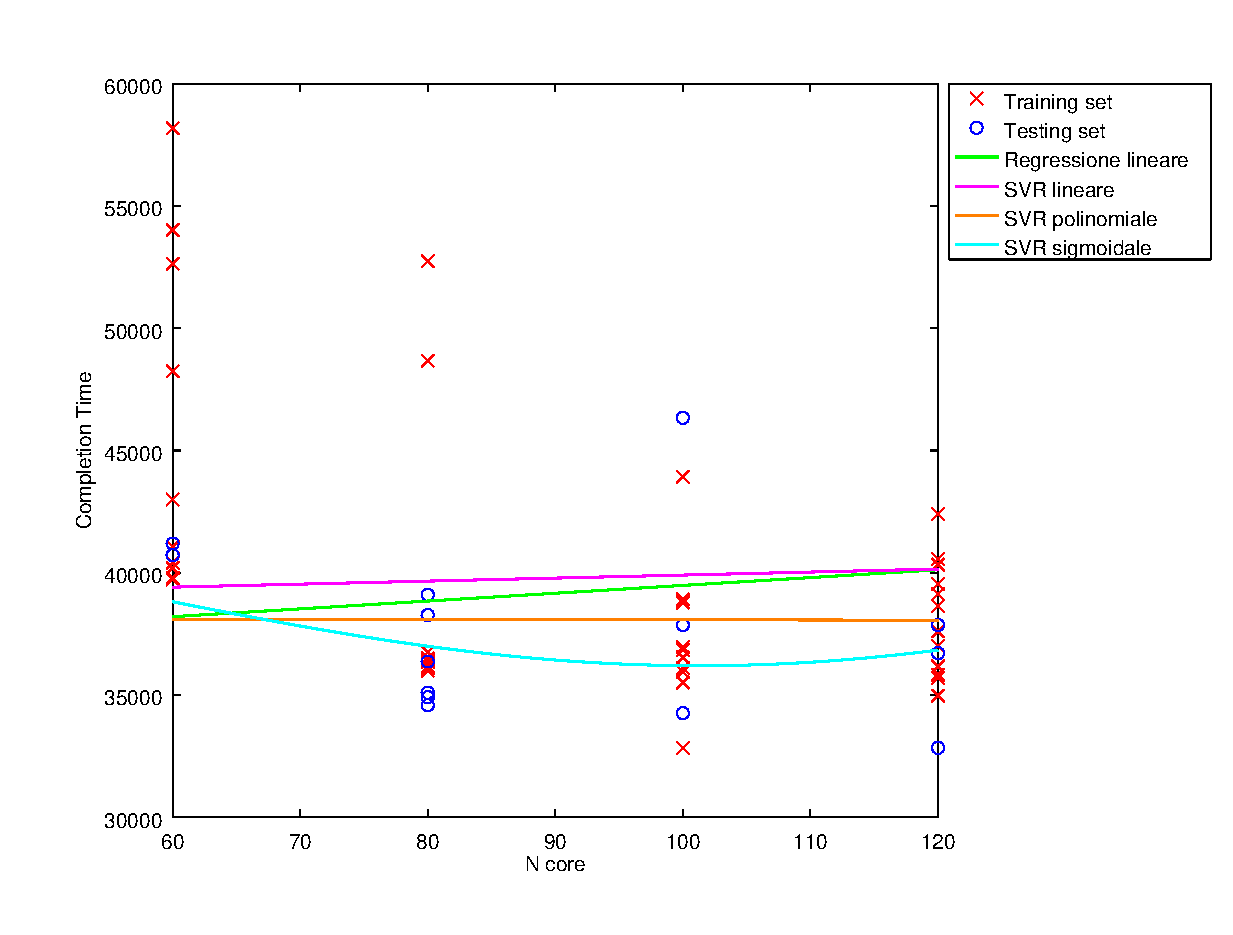
\includegraphics[width=\textwidth]{output/R5_1000/plot_R5_1000.eps}
\caption {Plot per il test su query R5 con datasize 1000}
\end {figure}

\newpage
\section{Fixed Cores}
\subsection{Query R1}
\subsubsection{Query R1 -- 60 cores}
\begin{table}[bhpt]
	\centering
	\begin{adjustbox}{center}
		\begin{tabular}{c | c M{1cm} M{2.5cm} M{2.5cm} M{1.8cm}}
			Modello & RMSE & R\textsuperscript{2} & Errore assoluto medio & Errore relativo medio \tabularnewline
			\hline
			Regressione lineare & 0.0992 & 0.9900 & 364573 & 0.8210 \\
			SVR lineare & 0.1036 & 0.9899 & 367989 & 0.1656 \\
			SVR polinomiale & 0.1528 & 0.9768 & 374847 & 0.3522 \\
			SVR sigmoidale & 0.2846 & 0.9356 & 383455 & 2.6615 \\
		\end{tabular}
	\end{adjustbox}
	\\
	\caption{Risultati per il test su query R1 con 60 cores}
	\label{table_R1_60cores}
\end{table}

\begin {figure}[hbtp]
\centering
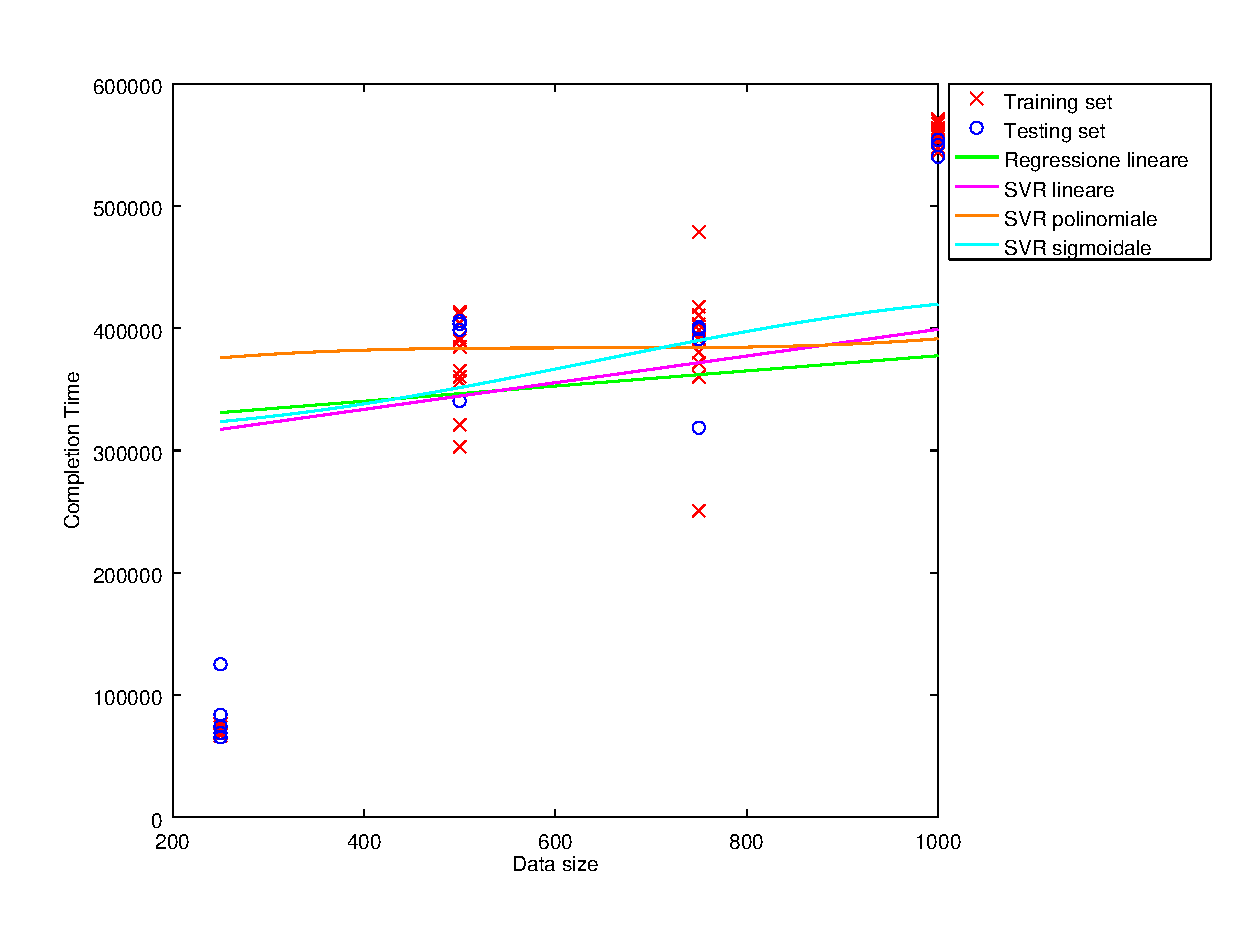
\includegraphics[width=\textwidth]{output/R1_60CORES/plot_R1_60CORES.eps}
\caption {Completion time vs Data size (R1 con 60 cores)}
\end {figure}
\newpage
\subsubsection{Query R1 -- 80 cores}
\newpage
\subsubsection{Query R1 -- 100 cores}
\newpage
\subsubsection{Query R1 -- 120 cores}
\newpage
\subsection{Query R2}
\subsubsection{Query R2 -- 60 cores}
\newpage
\subsubsection{Query R2 -- 80 cores}
\newpage
\subsubsection{Query R2 -- 100 cores}
\newpage
\subsubsection{Query R2 -- 120 cores}
\newpage
\subsection{Query R3}
\subsubsection{Query R3 -- 60 cores}
\newpage
\subsubsection{Query R3 -- 80 cores}
\newpage
\subsubsection{Query R3 -- 100 cores}
\newpage
\subsubsection{Query R3 -- 120 cores}
\newpage
\subsection{Query R4}
\subsubsection{Query R4 -- 60 cores}
\newpage
\subsubsection{Query R4 -- 80 cores}
\newpage
\subsubsection{Query R4 -- 100 cores}
\newpage
\subsubsection{Query R4 -- 120 cores}
\newpage
\subsection{Query R5}
\subsubsection{Query R5 -- 60 cores}
\newpage
\subsubsection{Query R5 -- 80 cores}
\newpage
\subsubsection{Query R5 -- 100 cores}
\newpage
\subsubsection{Query R5 -- 120 cores}

\end{document}
